% ===================================================================
%  数据存储的物理基础
%  Physical Foundations of Data Storage
%  物理学渣小微 · 重庆大学物理学院
% ===================================================================
\documentclass[11pt,a4paper,openany]{book}

% ===== Encoding & Fonts =====
\usepackage[UTF8]{ctex}
\usepackage[T1]{fontenc}
\usepackage{amsthm}
\usepackage{newtxtext,newtxmath}
\usepackage[scaled=0.92]{helvet}
\usepackage{courier}

% ===== Layout =====
\usepackage[margin=2.5cm,top=3cm,bottom=2.8cm,inner=3cm,outer=2cm]{geometry}
\usepackage{setspace}
\usepackage{fancyhdr}
\pagestyle{fancy}\fancyhf{}
\fancyhead[LE]{\small\itshape 数据存储的物理基础}
\fancyhead[RO]{\small\itshape\leftmark}
\fancyfoot[CE,CO]{\thepage}
\renewcommand{\headrulewidth}{0.4pt}

% ===== Math & Physics =====
\usepackage{amsmath,amsfonts,mathtools,bm,physics}
\usepackage{siunitx}
\sisetup{separate-uncertainty,per-mode=symbol}
\newcommand{\degC}{\ensuremath{{}^{\circ}\mathrm{C}}}
\DeclareSIUnit{\angstrom}{\text{\AA}}

% ===== Graphics =====
\usepackage{graphicx,xcolor}
\graphicspath{{./figures/}}
\usepackage{tikz,tikz-3dplot}
\usetikzlibrary{arrows.meta,shapes,decorations.pathmorphing,patterns,calc,positioning}
\usepackage{pgfplots}\pgfplotsset{compat=1.18}
\usepackage{float,circuitikz}

% ===== Tables =====
\usepackage{array,booktabs,tabularx,multirow,colortbl}

% ===== Hyperlinks =====
\usepackage[hidelinks,colorlinks=true,linkcolor=blue!60!black,citecolor=green!50!black,urlcolor=blue!60!black]{hyperref}
\usepackage[capitalise,nameinlink,noabbrev]{cleveref}

% ===== Custom Envs =====
\theoremstyle{definition}
\newtheorem{definition}{定义}[chapter]
\theoremstyle{plain}
\newtheorem{theorem}{定理}[chapter]
\newtheorem{lemma}[theorem]{引理}
\theoremstyle{remark}
\newtheorem{remark}{注解}[chapter]

\usepackage{tcolorbox}\tcbuselibrary{skins,breakable}
\newtcolorbox{physbox}[1][]{colback=blue!3!white,colframe=blue!50!black,
  fonttitle=\bfseries,title=物理注释,breakable,#1}
\newtcolorbox{histbox}[1][]{colback=brown!3!white,colframe=brown!50!black,
  fonttitle=\bfseries,title=历史注记,breakable,#1}

% ===== Metadata =====
\title{{\Huge\bfseries 数据存储的物理基础}\\[12pt]
       {\Large 从结绳记事到量子隧穿}\\[20pt]
       {\normalsize Physical Foundations of Data Storage:\\
        From Knot Records to Quantum Tunneling}}
\author{{\large 物理学渣小微}\\[4pt]
        {\normalsize 重庆大学物理学院}}
\date{2026年6月}

\raggedbottom
\begin{document}

% ===================================================================
\maketitle
\thispagestyle{empty}

\vspace*{6cm}
\begin{center}
{\small 献给所有对「信息何以存于物质」感到好奇的读者}
\end{center}
\newpage

% ===================================================================
\chapter*{自序}
\addcontentsline{toc}{chapter}{自序}

我始终着迷于一个看似简单的问题：当我们在计算机上点击「保存」并关闭电源后，
那些二进制的「0」和「1」到底去了哪里？它们以什么样的物理形态存在于物质世界中？
当我们在键盘上按下「删除」键，那些信息真的消失了吗——就像从未存在过一样？

这些问题将我引向了一条跨越磁学、半导体物理、量子力学、统计物理和信息论的漫长探索之路。
在这条路上，我逐渐认识到：\textbf{数据存储的每一个环节——写入、读取、保持、擦除——
都扎根于深刻的物理原理}。千亿个纳米磁畴在不足十毫秒内被精确翻转（硬盘写入）；
数万亿个电子通过薄至几十个原子层的氧化物势垒完成量子隧穿（闪存编程）；
聚焦至亚微米的激光脉冲在纳秒内将硫系合金从晶态熔化并急冷为非晶态（光盘刻录）。

理解这些过程所需的物理工具箱——从Heisenberg交换作用到Landauer擦除极限，
从Fowler-Nordheim隧穿的WKB推导到Stoner-Wohlfarth翻转的astroid几何——
恰好都在物理学本科四大力学和固体物理的射程之内。这正是我写作本书的初衷：
\textbf{用物理系学生熟悉的语言，讲述存储技术背后的第一性原理}。

本书的结构围绕六条物理主线展开。第1章从信息与物质的关系出发，梳理从结绳、泥板、
打孔卡到磁芯存储器的历史脉络，引出信息编码的物理学本质——将抽象的比特映射为
物质世界中两个（或多个）稳定可区分的微观状态。第2章至第5章分别阐述磁性存储、
半导体电荷存储、光子存储和新兴存储技术的物理原理。第6章将全部物理知识汇聚
至一个核心问题：\textbf{为什么「删除」不等于」物理消除」？}——
从磁畴剩磁的MFM探测、FTL异地更新的物理残留窗口，
到Landauer原理给出的擦除最小能耗（$k_B T\ln 2 \approx 18$ meV/bit）。

本书适合物理专业高年级本科生和研究生阅读。默认读者熟悉四大力学和固体物理的基本概念，
但每一章的关键物理推导均从第一性原理出发，力求自包含。

在写作中我遵循一条原则：\textbf{凡有公式，必给来历；凡有数值，必给估算}。
物理学的力量在于定量的预言和解释——写磁场需要多少kOe？浮栅中少了一个电子，
阈值电压偏多少毫伏？单次覆写后剩磁的信噪比是多少dB？数值使得这些物理概念不再悬浮于
抽象的理论天空，而是牢牢扎根于可测量、可验证的实验大地。

\vspace{1cm}
\begin{flushright}
物理学渣小微\\
重庆大学物理学院\\
2026年6月
\end{flushright}

\newpage

\tableofcontents

% ===================================================================
% CHAPTER 1
% ===================================================================
\chapter{信息与物质——存储的物理本质}
\label{ch:information}

\section{信息需要载体}

1948年，Claude Shannon发表了《通信的数学理论》，将信息定义为「不确定性的消除」。」
但Shannon的信息论——尽管天才般地为通信系统建立了数学框架——有意搁置了一个根本
问题：信息的物理载体是什么？Shannon自己写道：

\begin{quote}\itshape
The fundamental problem of communication is that of reproducing at one point
either exactly or approximately a message selected at another point.
Frequently the messages have \textbf{meaning}... These semantic aspects of
communication are irrelevant to the engineering problem.
\end{quote}

「工程问题」可以不关心语义，但\textbf{存储问题}不能回避物理。因为存储——
不同于通信——要求信息在时间中而非空间中保持。存储系统必须回答：
\begin{enumerate}
  \item 信息以何种物理量编码？\quad（磁化方向？电荷数？反射率？）
  \item 该物理量如何抵抗热涨落而长期稳定？\quad（能垒 $E_B \gg k_B T$）
  \item 如何可控地改变该物理量？\quad（写入/擦除）
  \item 如何在不破坏该物理量的前提下检测它？\quad（读取）
\end{enumerate}

这四个问题构成了贯穿全书的物理逻辑。本章从历史视角审视人类如何逐步将信息「存入」物质，
并建立信息编码的物理学一般框架。

\section{前电子时代：从泥板到打孔卡}

\subsection{苏美尔泥板与楔形文字（约公元前3400年）}

人类最早的持久信息存储介质是美索不达米亚的黏土泥板。
湿黏土被压实成板状，用芦苇笔（stylus）的楔形尖端在表面压出楔形印记——
这本质上是\textbf{塑性形变编码}：每个楔形印记改变黏土表面的局部几何形态，
产生稳定的、可见的物理对比度。

泥板的「写入」机制是压力诱导的塑性流动——黏土颗粒在应力超过屈服强度后不可逆地
重新排列。「读取」是可见光的散射对比——凹陷的楔形印记与平滑表面的散射差异肉眼可辨。
「保持」依赖于干燥黏土的机械强度——烧制后的泥板可在干旱气候中保存数千年
（大英博物馆藏有超过5000年历史的泥板）。

泥板的物理缺陷同样具有启示性：写入不可逆（一旦干燥，无法擦除塑性形变）；
密度极低（每平方厘米约一个楔形符号，相当于 $\sim 10^{-3}$ bit/mm$^2$）；
读取速度是「人类的阅读速度」。」

\subsection{纸张与墨水（约公元前3000年—至今）}

纸张的出现将信息载体从笨重的黏土解放为轻薄便携的纤维素薄膜。
墨水——无论是炭黑悬浮液（中国墨）还是铁-鞣酸络合物（中世纪欧洲铁胆墨水）——
在纸张纤维中沉积有色颗粒，产生\textbf{光学吸收对比度}。

从物理角度看，墨水的写入是液体在毛细作用下的渗透与表面附着——溶剂的蒸发将
颜料颗粒固定在纤维网格中。保持力取决于纤维素的水解速率和墨水的化学稳定性——
无酸纸+碳墨的组合在中性pH条件下可保存数百年。读取利用环境光在墨水区域（强吸收）
与纸张区域（漫反射）之间的反射率对比。

纸张的物理局限：写入速度受限于「人手运动+液体干燥」（约几个字符每秒），
密度受限于「人类视觉可分辨的字符尺寸」（约 $10$ bit/mm$^2$），
且\textbf{无法直接擦除后重用}（虽然可以刮去墨迹，但损伤纤维）。

\subsection{穿孔卡与穿孔带（1725年—1970年代）}

Basile Bouchon于1725年为提花织机发明了穿孔纸带——这是第一个「机器可读」
的存储格式。信息以\textbf{有孔/无孔}的二进制方式编码在卡纸的离散位置上。

从信息存储的物理视角审视，穿孔卡是一次质的飞跃：它是第一个真正的
\textbf{离散数字存储介质}——每个比特对应一个物理上不连续的、独立可区分的状态。
「1」 = 有孔（光/气流通），「0」 = 无孔（光/气流阻断）。
读取不再依赖人类视觉，而是通过机械探针或光电传感器自动检测。

Herman Hollerith的1890年美国人口普查打孔卡奠定了现代数据处理的基础，
其80列$\times$12行的格式在IBM系统中沿用至1980年代。
一张标准打孔卡携带 $80 \times 12 = 960$ bit $\approx 120$ byte的数据——
即每平方厘米约1字节。

\begin{histbox}
\textbf{打孔卡的物理隐喻。}打孔卡蕴含了一个至今指导存储设计的物理原则：
信息编码为\textbf{两个具有足够对比度的稳定物理状态}。「有孔」状态通过机械去除
局部材料实现——这在热力学上是不可逆的（除非填补孔洞）。因此打孔卡天然是
「一次写入多次读取」（Write-Once Read-Many, WORM）介质——
这与后来光学存储中的CD-R/DVD-R在物理逻辑上一脉相承。
\end{histbox}

\section{电磁时代的曙光：磁芯存储器}

1949年，MIT的Jay Forrester为Whirlwind计算机发明了磁芯存储器——第一个
实用的随机存取电子存储设备。磁芯存储器的物理原理预示了后来硬盘驱动器的核心机制：
\textbf{利用铁磁材料的磁滞回线编码二进制信息}。

磁芯是一个环形铁氧体（铁磁陶瓷，通常为(Mn,Zn)Fe$_2$O$_4$），外径约
$1$--$2$ mm。穿过磁芯的导线通以电流产生环形磁场。当电流超过阈值时，
磁芯沿该磁场方向饱和磁化；电流撤去后，剩余磁化强度$M_r$保持——该方向编码了
「0」或「1」。」读取时施加一个「尝试写入」脉冲——若磁芯的磁化发生翻转
（感应出较大的读出信号），则原状态与脉冲方向相反（即「1」）；
若磁芯未翻转（感应信号小），则原状态与脉冲方向相同（即「0」）。
注意这一读取是\textbf{破坏性}的——读后必须重写。

Forrester的磁芯存储器在1953年首次部署于Whirlwind，随后成为1950--1970年代
几乎所有大型计算机（包括阿波罗登月导航计算机）的标准主存。
典型的磁芯存储器板（约 $30 \times 30$ cm$^2$）可存储约 $32 \times 32 \times 16
\approx 16$ Kbit。这约等于2 KB——但在1953年，这是革命性的。

磁芯存储器揭示了磁性存储的两个核心物理事实，至今仍然成立：
\begin{enumerate}
  \item \textbf{铁磁材料的磁滞回线是自然的二进制存储单元}——两个剩余磁化状态
  $\pm M_r$ 在没有外场时稳定存在，弛豫时间随$K_u V/k_B T$呈指数增长。
  \item \textbf{读取与写入的能量代价不对称}——破坏性读取需要每次读后重写，
  但在后来的硬盘中，TMR读头实现了无损读取，使得「读」的边际能耗远低于」写」。」
\end{enumerate}

磁芯存储器于1970年代被半导体DRAM和SRAM取代，但其物理原理直接传承至
硬盘驱动器（第2章）和磁阻RAM（第5章）。

\section{存储技术的统一物理框架}

回顾从泥板到磁芯的漫长历史，我们可以提炼出信息存储的\textbf{统一物理框架}：

\begin{definition}[信息存储的物理学定义]
信息存储是将一组抽象符号$\{s_i\}$映射为物理介质的一组可区分微观状态
$\{\psi_i\}$的过程。该映射必须满足：
\begin{enumerate}
  \item \textbf{非易失性（稳定性）}：态$\psi_i$在无外界干预时自发弛豫至其他态
  的特征时间$\tau$远大于预期的信息保留时间要求。
  物理条件：能垒$E_B \gg k_B T$，$\tau = \tau_0\exp(E_B/k_B T)$。
  \item \textbf{可写性（可控切换）}：存在一种方法，以合理的能量和时间
  将系统从$\psi_i$切换到$\psi_j$（$i \neq j$）。
  \item \textbf{可读性（无损探测）}：存在一种探针，可以区分$\psi_i$和$\psi_j$
  而不改变其状态。
\end{enumerate}
\end{definition}

表\ref{tab:carrier-history}总结了人类历史上主要信息载体的物理机制。

\begin{table}[H]
\centering
\caption{信息载体的物理演变}
\begin{tabular}{@{}lcccc@{}}
\toprule
载体 & 编码物理量 & 写入机制 & 面密度 & 擦除能力 \\
\midrule
泥板 & 表面几何形变 & 塑性流动 & $\sim 10^{-3}$ bit/mm$^2$ & 不可擦 \\
纸张+墨水 & 光学吸收 & 毛细渗透+蒸发 & $\sim 10$ bit/mm$^2$ & 不可擦 \\
打孔卡 & 有/无孔 & 机械冲压 & $\sim 8$ bit/mm$^2$ & 不可擦 \\
磁芯 & 磁化方向 & 磁场翻转 & $\sim 1$ bit/mm$^2$ & 可重写 \\
HDD & 磁畴方向 & 写磁头磁场 & $\sim 10^9$ bit/mm$^2$ & 可重写 \\
NAND闪存 & 浮栅电荷 & 量子隧穿 & $\sim 10^9$ bit/mm$^2$ & 块擦除 \\
光盘(ROM) & 反射率坑 & 压模成型 & $\sim 10^7$ bit/mm$^2$ & 不可擦 \\
\bottomrule
\end{tabular}
\label{tab:carrier-history}
\end{table}

从苏美尔泥板到3D NAND闪存，信息密度的提升跨越了约12个数量级——从
$10^{-3}$到$10^9$ bit/mm$^2$。这一飞跃由两项平行革命驱动：
\textbf{物理学革命}（从宏观塑性到纳米磁畴和量子隧穿的尺度跨越）
和\textbf{工程学革命}（从人手书写到光刻和原子层沉积的制造精度跨越）。
本书的后续章节将深入探讨支撑当前最高密度存储技术的物理原理。

% ===================================================================
% CHAPTER 2
% ===================================================================
\chapter{磁性存储物理}
\label{ch:magnetic}

\section{从磁芯到硬盘}

第1章末尾讨论的磁芯存储器使用宏观环形铁氧体（$\sim 1$ mm尺度）作为存储单元。
硬盘驱动器将这一物理原理推向了极致：将信息存储从毫米尺度的离散磁环
缩小到纳米尺度的连续多晶薄膜，每个比特由约10--20个直径6--10 nm的晶粒
的集体磁化方向编码。这一尺度跨越——从宏观到纳米——使得面密度从
$\sim 1$ bit/mm$^2$提升至超过$10^9$ bit/mm$^2$（即超过1 Tb/in$^2$），
提升了九个数量级。

推进这一跨越的物理学问题，恰好构成了一个完整的凝聚态物理课程：
铁磁性的量子力学起源、磁各向异性的自旋-轨道耦合微观理论、
磁化翻转的非线性动力学（LLG方程）、热激活弛豫的统计物理（Arrhenius-N\'{e}el理论）、
以及自旋极化输运的量子理论（TMR效应）。

\section{铁磁性的量子起源}

\subsection{Heisenberg交换作用}

铁磁性的本质是多体量子效应——Coulomb排斥与Pauli不相容原理的协同产物。
这一定性陈述可以追溯到1928年Heisenberg的奠基性工作。

考虑两个相邻原子的局域d电子（自旋分别为$\mathbf{S}_1$和$\mathbf{S}_2$）。
Coulomb相互作用$e^2/r_{12}$通过波函数的交换反对称性产生了与自旋取向相关的能量差。
在Heisenberg模型中，该能量差被捕捉为各向同性的自旋-自旋耦合：
\begin{equation}\label{eq:heisenberg}
  \mathcal{H}_{\text{ex}} = -J \sum_{\langle i,j\rangle} \mathbf{S}_i \cdot \mathbf{S}_j
  = -J \sum_{\langle i,j\rangle} \bigl[ S_i^z S_j^z
    + \tfrac{1}{2}(S_i^+ S_j^- + S_i^- S_j^+) \bigr]
\end{equation}
其中$J$为交换积分，求和限于最近邻。$J$由轨道的空间交叠和Coulomb排斥的
精细平衡决定。对于Co、Fe等3d过渡金属，$J \sim 10$--$20$ meV
（由局域自旋密度泛函理论（LSDA）计算得到）。

\textbf{交换积分的符号}决定了磁有序的类型：
\begin{itemize}
  \item $J > 0$：平行排列能量更低 $\to$ \textbf{铁磁性}（Fe, Co, Ni, 及它们的合金）
  \item $J < 0$：反平行排列能量更低 $\to$ \textbf{反铁磁性}（Mn, Cr, MnO, NiO）
\end{itemize}

交换积分的符号和大小与原子间距$R$和d轨道半径$r_d$之比$R/r_d$有关——
即\textbf{Bethe-Slater曲线}。当$R/r_d \gtrsim 3$时$J > 0$（铁磁）；当$R/r_d \lesssim 3$
时$J < 0$（反铁磁）。hcp Co的$R/r_d \approx 3.3$，恰好落在铁磁区的强耦合端。
这一简单规律解释了为何在元素周期表中，铁磁性仅出现在第一过渡系的中间几个
元素及其合金中——这是轨道空间延展性与Coulomb排斥竞争的直接结果。

\subsection{Heitler-London模型与交换积分的物理根源}

在自旋密度泛函理论（DFT）成为标准工具之前，Heitler和London（1927）通过
两个氢原子的问题揭示了交换作用的基本物理。

两个质子（$a$和$b$）和两个电子（1和2）的Hamiltonian为：
\begin{equation}
  \mathcal{H} = -\frac{\hbar^2}{2m_e}(\nabla_1^2 + \nabla_2^2)
  - \frac{e^2}{r_{1a}} - \frac{e^2}{r_{1b}} - \frac{e^2}{r_{2a}} - \frac{e^2}{r_{2b}}
  + \frac{e^2}{r_{12}}
\end{equation}
忽略核动能和核间排斥（假定核位置固定）。在分子轨道法的反对称化基矢下，
单重态（$S=0$，空间波函数对称）和三重态（$S=1$，空间波函数反对称）的能量差为：
\begin{equation}\label{eq:heitler-london}
  J_{\text{HL}} = \frac{1}{2}(E_S - E_T)
  = \frac{1}{1 - S_{ab}^2}\bigl[ K_{ab} - S_{ab} J_{ab} \bigr]
\end{equation}
各项的物理意义：
\begin{itemize}
  \item $S_{ab} = \langle a|b \rangle$：轨道交叠积分（$0 < S_{ab} < 1$）。
  \item $K_{ab} = \langle ab|1/r_{12}|ba \rangle$：\textbf{交换积分}——两个电子
  「交换」其轨道位置后的Coulomb期待值。这是纯粹的量子效应，无经典对应。
  \item $J_{ab} = \langle ab|1/r_{12}|ab \rangle$：直接Coulomb积分。
\end{itemize}

\textbf{铁磁性要求$K_{ab} > S_{ab}J_{ab}$}——即交换积分压倒交叠项。
在第一过渡系的3d元素中，d轨道的空间局域性（较小的$r_d$）意味着$S_{ab}$较小，
而$K_{ab}$因d轨道的高角动量和高Fermi面态密度而显著——
这些条件的组合使得Fe、Co、Ni成为自然界中仅有的室温铁磁性元素。

\subsection{Stoner巡游电子模型}

Heisenberg模型适用于局域磁矩体系（绝缘磁体，如铁氧体、稀土永磁）。
但对于金属铁磁体——Fe、Co、Ni及其合金——磁性d电子并非局域在单个原子上，
而是占据扩展的Bloch态。需要\textbf{Stoner巡游电子模型}（1938）。

在Stoner图像中，铁磁性源自自旋向上和自旋向下的能带因交换关联而发生
\textbf{刚性相对位移}——交换劈裂$\Delta E_{\text{ex}}$。
设自旋向上（$\uparrow$）和自旋向下（$\downarrow$）能带的电子占有数分别为
$n_\uparrow$和$n_\downarrow$：
\begin{align}
  n_\uparrow &= \int_{-\infty}^{E_F} D\left(E - \frac{\Delta E_{\text{ex}}}{2}\right)\,dE
  \label{eq:stoner-nup} \\
  n_\downarrow &= \int_{-\infty}^{E_F} D\left(E + \frac{\Delta E_{\text{ex}}}{2}\right)\,dE
  \label{eq:stoner-ndown}
\end{align}
净磁矩$m = n_\uparrow - n_\downarrow$（以$\mu_B$为单位）。自洽性要求交换劈裂与
磁矩成正比：$\Delta E_{\text{ex}} = I m$，其中$I$为\textbf{Stoner交换参数}
（对于Co，$I \approx 0.9$ eV）。

对$m \ll 1$展开，在Fermi能级附近：
\begin{equation}\label{eq:stoner-criterion}
  m \approx D(E_F)\, \Delta E_{\text{ex}} = I D(E_F) \, m
\end{equation}
非平凡解$m \neq 0$存在的条件即为\textbf{Stoner判据}：
\begin{equation}
  \boxed{ I \cdot D(E_F) > 1 }
\end{equation}

\begin{physbox}
\textbf{数值检验。}对于hcp Co：
Fermi能级处的态密度$D(E_F) \approx 1.8$ eV$^{-1}$（由第一性原理LSDA能带计算给出），
Stoner交换参数$I \approx 0.9$ eV。
$I D(E_F) \approx 1.62 > 1$——满足Stoner判据，且余量充裕。
相比之下，fcc Pd的$I D(E_F) \approx 0.9 < 1$——近乎铁磁但尚未满足判据
（即Stoner增强因子$(1 - I D(E_F))^{-1} \approx 10$——解释了Pd的巨Pauli顺磁性）。

\textbf{Slater-Pauling曲线}总结了3d铁磁合金的原子磁矩随平均价电子数的变化。
在强铁磁体中，多数自旋d带完全填满（约5个电子/原子），少数自旋d带的填充分数
随价电子数线性变化。Co$(Z=27)$的价电子构型$3d^8 4s^1$（固体中约为$3d^{8.3} 4s^{0.7}$），
磁矩$\approx 1.72\ \mu_B$/atom——位于Slater-Pauling曲线的峰值附近。
这是Co基合金（CoCrPt, CoFe, CoFeB）广泛用于磁记录技术的最底层电子结构原因。
\end{physbox}

\section{微磁学：连续介质中的磁化理论}

\subsection{交换长度与连续近似}

在磁记录介质的空间尺度（纳米至微米）上，原子尺度的离散自旋模型过于精细而
在计算上不可行。微磁学（Brown, 1963）提供了恰当的连续介质描述：
将磁化矢量视为位置的光滑函数$\mathbf{M}(\mathbf{r})$，其模长
$|\mathbf{M}(\mathbf{r})| = M_s$（饱和磁化强度）在低于$T_C$时近似恒定，
而\textbf{方向}$\mathbf{m}(\mathbf{r}) = \mathbf{M}(\mathbf{r})/M_s$是空间坐标
的连续函数。

这一近似的合法性依赖于\textbf{交换长度}：
\begin{equation}
  l_{\text{ex}} = \sqrt{\frac{A}{K_u}}
\end{equation}
其中$A \approx J S^2 z / (2a)$为交换刚度常数（$z$为配位数，$a$为晶格常数）。
对于hcp Co，$A \approx 3.0 \times 10^{-11}$ J/m，$K_u \approx 4.5 \times 10^5$ J/m$^3$，
$l_{\text{ex}} \approx 8$ nm$\gg$原子间距（$\sim 0.25$ nm）。
连续近似合法：在交换长度的尺度内，数千个原子自旋已完成了方向的平滑过渡。

\subsection{磁自由能泛函的五项分解}

在微磁学框架中，系统的总磁Gibbs自由能是磁化方向场$\mathbf{m}(\mathbf{r})$
的泛函，可分解为五个物理来源不同的贡献：
\begin{equation}\label{eq:free-energy}
  E_{\text{total}}[\mathbf{m}]
  = E_{\text{ex}} + E_{\text{ani}} + E_{\text{demag}} + E_{\text{Zeeman}} + E_{\text{DMI}}
\end{equation}

\subsubsection{交换能}

在连续极限下，$\mathbf{m}$的空间梯度导致交换能的升高（类似于非线性$\sigma$模型的梯度项）：
\begin{equation}\label{eq:exchange}
  E_{\text{ex}} = A\int_V (\nabla\mathbf{m})^2\,d^3r
  = A\int_V \bigl[ (\nabla m_x)^2 + (\nabla m_y)^2 + (\nabla m_z)^2 \bigr]\,d^3r
\end{equation}
交换能倾向于$\nabla\mathbf{m} = 0$（均匀磁化），但交换作用本身是各向同性的——
它不能单独确定磁化的\textbf{方向}，仅对磁化的\textbf{空间变化}施加了能量代价。

\subsubsection{磁晶各向异性能}

自旋-轨道耦合$\mathcal{H}_{\text{SO}} = \xi \mathbf{L}\cdot\mathbf{S}$
将各向同性的自旋系统「钉扎」到晶格的方向上。在hcp Co中，c轴（$[0001]$方向）
是易磁化轴——沿该方向磁化时的能量最低。对于垂直磁记录介质（CoCrPt合金），
织构化的c轴垂直于膜面。

在单轴各向异性的最简单近似下：
\begin{equation}\label{eq:anisotropy}
  E_{\text{ani}} = K_u\int_V \sin^2\theta(\mathbf{r})\,d^3r
\end{equation}
其中$\theta$为$\mathbf{m}$与易磁化轴的夹角。
$K_u$有三个微观贡献：

\textbf{(1) 磁晶各向异性}——体贡献。在hcp Co中，$K_1^{\text{bulk}} \approx 4.5 \times 10^5$ J/m$^3$。
其电子结构起源是最低阶的单离子各向异性：Co$^{2+}$离子（$3d^7$）在hcp晶场中，
轨道角动量部分猝灭（$L_z \neq 0$），自旋-轨道耦合将磁矩钉扎在c轴。

\textbf{(2) 界面（N\'{e}el）各向异性}——在多层膜中（如Co/Pt或Co/Pd），
界面处Co原子配位环境不对称：一侧为本体Co，另一侧为重金属（Pt、Pd）。
N\'{e}el（1954）提出界面各向异性来源于原子对方向的各向异性键。
对于Co/Pt界面，$K_s \approx 1$--$2$ mJ/m$^2$。
当Co层厚度$t_{\text{Co}} < 1$ nm时，界面贡献通过$K_u^{\text{eff}} = K_u^{\text{bulk}} + 2K_s/t_{\text{Co}}$
压倒体贡献，有效各向异性显著增强。

\textbf{(3) 磁弹各向异性}——薄膜生长中的残余应力通过磁致伸缩耦合到磁化方向。
$\Delta K_{\text{me}} = \frac{3}{2}\lambda_s\sigma$，
其中$\lambda_s$为饱和磁致伸缩常数（CoCrPt: $\lambda_s \approx -2 \times 10^{-5}$），
$\sigma$为面内应力。

\subsubsection{退磁能}

退磁能是磁偶极-偶极长程相互作用的连续极限。
磁化体内的等效「磁荷」密度为$\rho_m = -\nabla \cdot \mathbf{M}$，
面磁荷密度$\sigma_m = \mathbf{M}\cdot\hat{n}$。退磁场由磁标势的梯度给出：
\begin{align}
  \mathbf{H}_d &= -\nabla\phi_M, \quad
  \nabla^2\phi_M = \nabla\cdot\mathbf{M}
  \label{eq:poisson-mag}
\end{align}
退磁能密度为：
\begin{equation}\label{eq:demag}
  \varepsilon_{\text{demag}} = -\frac{\mu_0}{2}\mathbf{M}\cdot\mathbf{H}_d
\end{equation}
对于垂直磁化的无限大薄板（厚度$t$），退磁场在板内近似均匀：
$\mathbf{H}_d = -M_s\hat{z}$，$\varepsilon_{\text{demag}} = \frac{1}{2}\mu_0 M_s^2$。

正是退磁能的这一正值使垂直磁化在能量上不利——形状各向异性倾向于拉回面内。
\textbf{垂直磁记录之所以可行，仅因为磁晶各向异性$K_u$压倒了退磁能。}
垂直记录介质的第一个设计判据：
\begin{equation}\label{eq:keff}
  K_{\text{eff}} = K_u - \frac{1}{2}\mu_0 M_s^2 > 0
\end{equation}
对于CoCrPt-氧化物薄膜，$M_s \approx 3.0 \times 10^5$ A/m，
$\frac{1}{2}\mu_0 M_s^2 \approx 5.7 \times 10^4$ J/m$^3$，
$K_{\text{eff}} \approx 1.4 \times 10^5$--$4.4 \times 10^5$ J/m$^3 > 0$。

\subsubsection{Zeeman能与Dzyaloshinskii-Moriya相互作用}

Zeeman能：$E_{\text{Zeeman}} = -\mu_0\int \mathbf{M}\cdot\mathbf{H}_{\text{ext}}\,d^3r$，
是外磁场写入的驱动源。

Dzyaloshinskii-Moriya相互作用（DMI）：
$E_{\text{DMI}} = D\int [m_z(\nabla\cdot\mathbf{m}) - (\mathbf{m}\cdot\nabla)m_z]\,d^3r$，
来源于空间反演对称性的破缺+自旋-轨道耦合。在传统HDD介质中DMI是非主导项
（$D \ll \sqrt{AK_u}$），但在赛道存储器（racetrack memory）和磁斯格明子中有核心作用。

\subsection{有效场与Landau-Lifshitz-Gilbert方程}

由能量泛函对$\mathbf{M}$取泛函导数（保持$|\mathbf{m}| = 1$约束），
得到\textbf{有效场}：
\begin{equation}
  \mathbf{H}_{\text{eff}} = -\frac{1}{\mu_0}\frac{\delta E_{\text{total}}}{\delta\mathbf{M}}
  = \mathbf{H}_{\text{ext}} + \mathbf{H}_d + \frac{2A}{\mu_0 M_s^2}\nabla^2\mathbf{m}
  + \frac{2K_u}{\mu_0 M_s^2}(\mathbf{m}\cdot\hat{u})\hat{u} + \cdots
\end{equation}

磁化动力学由\textbf{Landau-Lifshitz-Gilbert（LLG）方程}描述——
这是微磁学的基本动力学方程，也是所有磁化翻转模拟的出发点：
\begin{equation}\label{eq:llg}
  \boxed{
  \frac{\partial\mathbf{M}}{\partial t}
  = -\gamma\mathbf{M}\times\mathbf{H}_{\text{eff}}
  + \frac{\alpha}{M_s}\mathbf{M}\times\frac{\partial\mathbf{M}}{\partial t}
  }
\end{equation}
其中：
\begin{itemize}
  \item $\gamma = g\mu_B/\hbar \approx 1.761 \times 10^{11}$ rad/(s$\cdot$T)——
  自由电子旋磁比。对于Co，$g \approx 2.17$（轨道角动量未完全猝灭），
  $\gamma_{\text{Co}} \approx 1.91 \times 10^{11}$ rad/(s$\cdot$T)。
  \item $\alpha \approx 0.02$--$0.05$为Gilbert阻尼常数。
  阻尼的微观来源是自旋-轨道耦合将进动能量传递给声子（晶格振动），以热的形式耗散。
\end{itemize}

\textbf{LLG方程的物理图像}：
\begin{itemize}
  \item 第一项（进动项）：$\mathbf{M}$绕$\mathbf{H}_{\text{eff}}$做Larmor进动，
  角频率$\omega = \gamma H_{\text{eff}}$。在$H_{\text{eff}} = 1$ T下，
  $\omega \approx 28$ GHz（微波范围）。该项是保守的（不改变系统的总能量）。
  \item 第二项（阻尼项）：将进动能量耗散为热，使$\mathbf{M}$逐渐趋于
  $\mathbf{H}_{\text{eff}}$的方向——即磁自由能的局部极小点。
  阻尼使「围绕易轴的进动」以时间常数$1/(\alpha\gamma H_K)$衰减。
\end{itemize}

\section{磁化翻转的Stoner-Wohlfarth理论}

\subsection{单畴粒子与相干翻转}

当晶粒尺寸$d < l_{\text{ex}}$（$\sim 8$ nm）时，交换能远大于退磁能的空间变化，
所有原子自旋被迫\textbf{一致旋转}——即相干翻转。
Stoner和Wohlfarth（1948）在此假设下获得了单畴粒子磁化翻转的精确解析解。

对于一个单轴各向异性的椭球粒子，磁化$\mathbf{m}$与易轴（设为$z$方向）的夹角为$\theta$，
外磁场$\mathbf{H}$与易轴的夹角为$\psi$。单位体积的磁能为：
\begin{equation}\label{eq:sw-energy}
  \varepsilon(\theta) = K_u\sin^2\theta - \mu_0 M_s H\cos(\theta - \psi)
\end{equation}
第一项为各向异性能（两处极小：$\theta = 0, \pi$），第二项为外场能。

平衡条件$\partial\varepsilon/\partial\theta = 0$：
\begin{equation}\label{eq:sw-equilibrium}
  2K_u\sin\theta\cos\theta + \mu_0 M_s H\sin(\theta - \psi) = 0
\end{equation}
稳定性条件$\partial^2\varepsilon/\partial\theta^2 > 0$。

引入无量纲场$\mathbf{h} = \mathbf{H}/H_K$（$H_K = 2K_u/(\mu_0 M_s)$为各向异性场）。
在$h_x$-$h_z$平面上（外场在$xz$平面内），稳定性边界构成一条四尖点星形线——
\textbf{Stoner-Wohlfarth Astroid}：
\begin{equation}\label{eq:astroid}
  \boxed{ h_x^{2/3} + h_z^{2/3} = 1 }
\end{equation}

\begin{figure}[htbp]
\centering
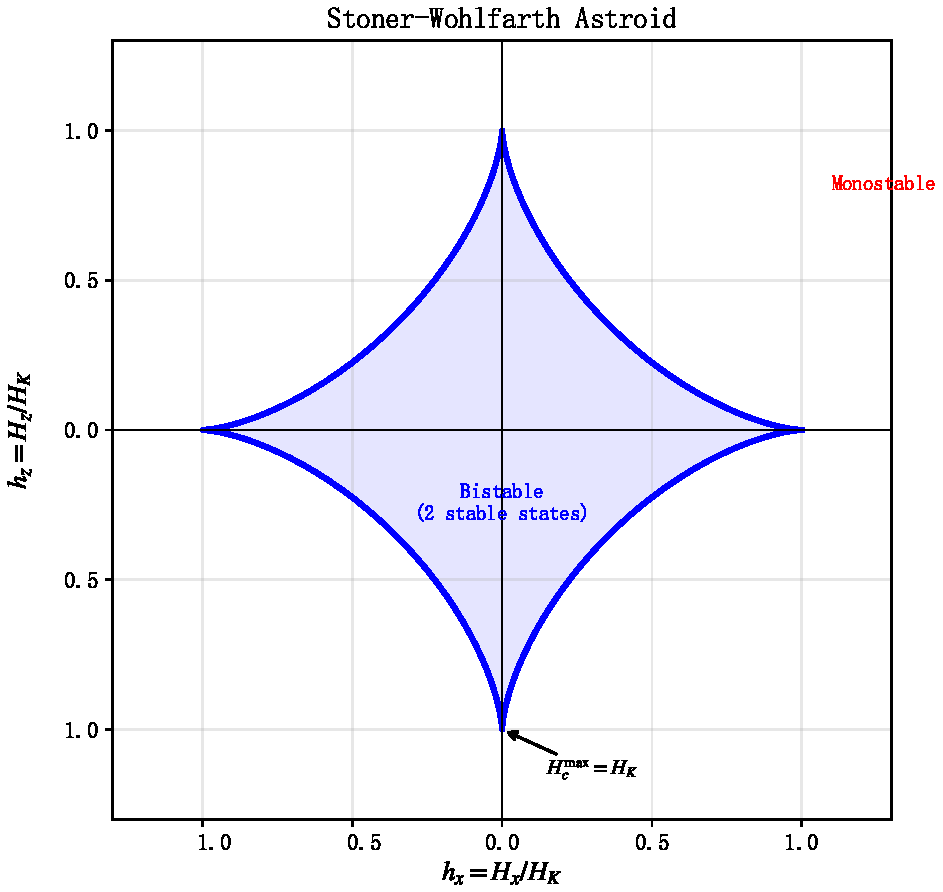
\includegraphics[width=0.48\textwidth]{fig-astroid}
\hspace{0.04\textwidth}
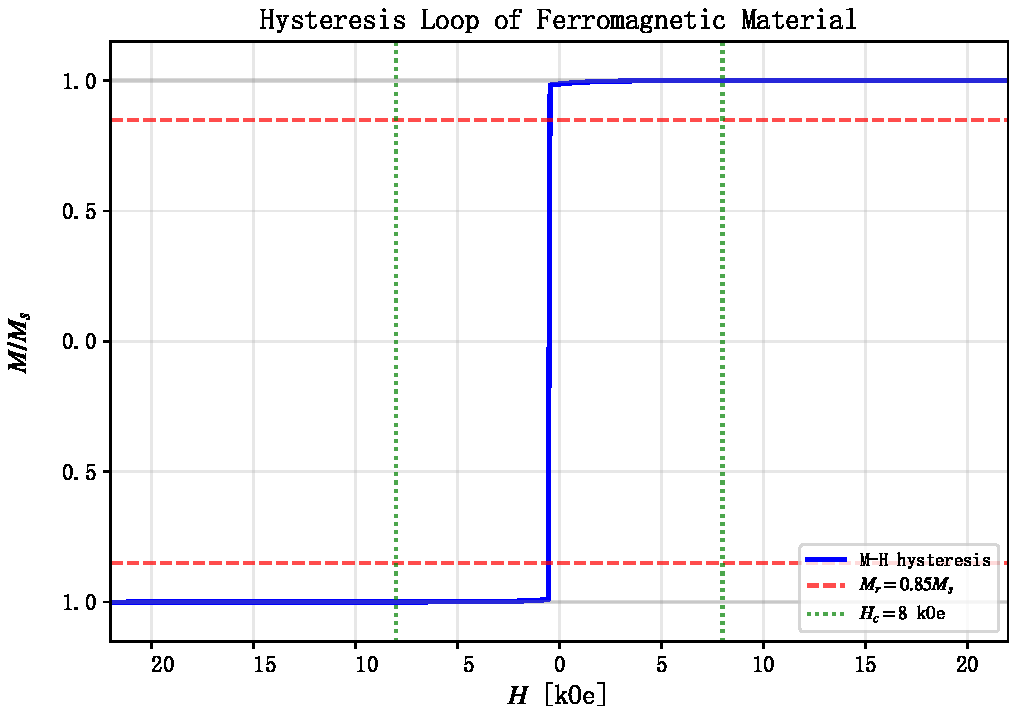
\includegraphics[width=0.48\textwidth]{fig-hysteresis}
\caption{\textbf{左}：Stoner-Wohlfarth Astroid。曲线内部为双稳态（2个稳定磁化方向），
外部为单稳态。当外场矢量$\mathbf{H}$跨越Astroid时，磁化发生不可逆翻转。
沿$-z$方向的翻转所需的最大场为$H_K$（最「顽固」的晶粒取向）。
\textbf{右}：铁磁材料的磁滞回线。$M_r$为剩余磁化（外场归零后的可保持磁化），
$H_c$为矫顽力。矩形比$S = M_r/M_s$越接近1，两个存储态的区分度越好。}
\label{fig:sw-hysteresis}
\end{figure}

\textbf{Astroid的几何特征与工程含义}：
\begin{itemize}
  \item 沿$-z$（易轴反方向）：矫顽力取最大值$H_c^{\max} = H_K$。这是介质中晶粒
  抵抗无意翻转的最强方向——也是最难写入的方向。
  \item 沿与易轴呈$45^\circ$方向：矫顽力最小，$H_c^{\min} = H_K/2$。
  \item 在实际的多晶介质中，晶粒的易轴取向是分散的（织构分布），因此写磁头产生的
  场必须超过最坏情况下的$H_c^{\max}$以确保所有晶粒都被可靠翻转。
\end{itemize}

\subsection{磁记录的三元悖论}

Stoner-Wohlfarth理论直接导出了矫顽力$H_c$与各向异性$K_u$的正比关系。
结合N\'{e}el的热激活理论——翻转时间$\tau = \tau_0\exp(K_u V/k_B T)$，
要求$\tau > 10$年$\Rightarrow K_u V/k_B T \gtrsim 60$——我们得到
\textbf{磁记录的三元悖论（Magnetic Recording Trilemma）}：

\begin{enumerate}
  \item \textbf{更高面密度} $\to$ 比特尺寸缩小 $\to$ 每比特内的晶粒体积$V$减小
  （或晶粒数目减少，介质噪声恶化）。
  \item 更小的$V$意味着能垒$K_u V$下降。为维持$K_u V/k_B T > 60$（数据保持$>10$年），
  \textbf{必须增大$K_u$}。
  \item 但更大的$K_u$导致更高的矫顽力$H_c \propto K_u/M_s$。
  而写磁头尖端的最大磁场受限于软磁材料的饱和磁化强度——
  FeCo的$B_s \approx 2.4$ T已是已知最高值。
  \textbf{写磁头无法产生足以翻转超高$K_u$介质的写场}。
\end{enumerate}

\begin{figure}[htbp]
\centering
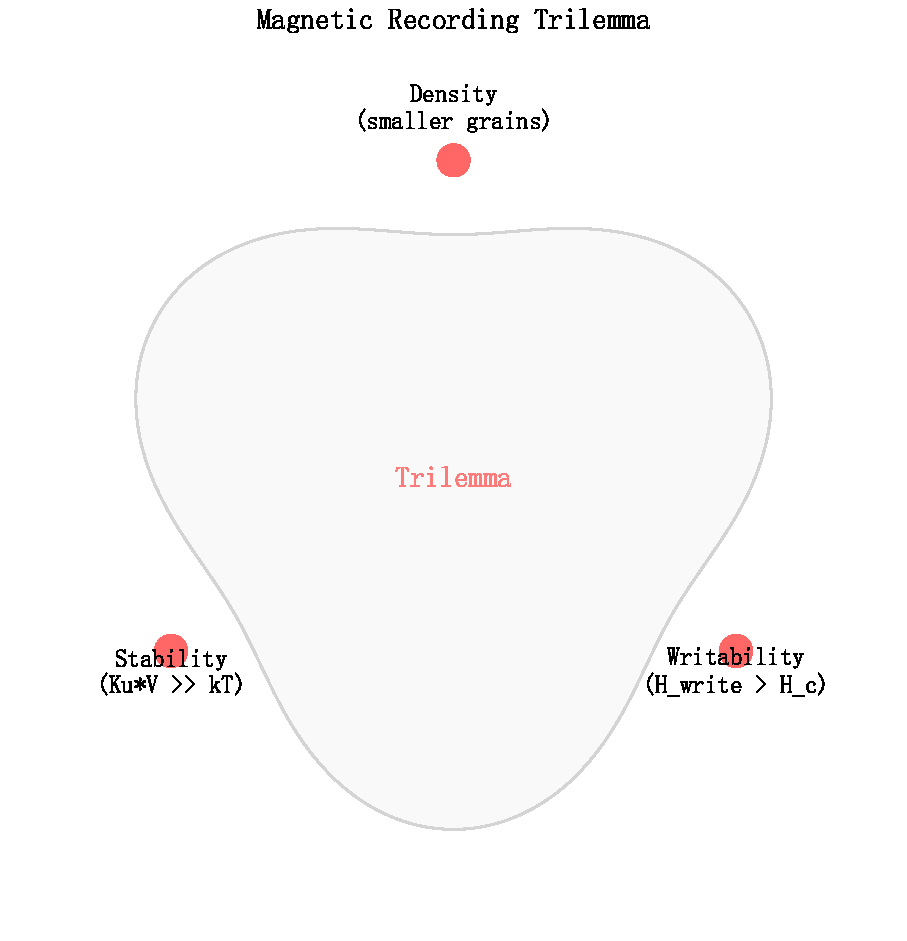
\includegraphics[width=0.45\textwidth]{fig-trilemma}
\caption{磁记录三元悖论：密度（小晶粒）、热稳定性（高能垒）、可写性（低矫顽力）
三者无法同时优化。HAMR通过瞬态降低矫顽力（加热介质至居里温度附近）打破这一悖论。}
\label{fig:trilemma}
\end{figure}

三元悖论直接推动了\textbf{热辅助磁记录（HAMR）}和\textbf{微波辅助磁记录（MAMR）}
技术的诞生。这两种方案都试图打破「高$K_u$ $\to$ 高$H_c$ $\to$ 不可写」的僵局——
HAMR通过加热瞬态降低$H_c$（见\S\ref{sec:hamr}），
MAMR通过在写场上叠加铁磁共振频率的微波来降低翻转能垒。

\subsection{Arrhenius-N\'{e}el热激活翻转}

在绝对零度下，当$H < H_K$时，磁化被各向异性能垒$K_u V$牢牢限制在势阱底部的
稳定方向。但在有限温度下，热涨落可以以概率$\propto \exp(-K_u V/k_B T)$克服能垒。
N\'{e}el（1949）建立了热激活翻转的Arrhenius定律：
\begin{equation}\label{eq:neel}
  \boxed{ \tau = \tau_0 \exp\!\left( \frac{K_u V}{k_B T} \right) }
\end{equation}
其中$\tau_0 \approx 10^{-9}$--$10^{-10}$ s为尝试时间
（约等于$\gamma H_K$决定的Larmor进动周期的倒数）。

\begin{figure}[htbp]
\centering
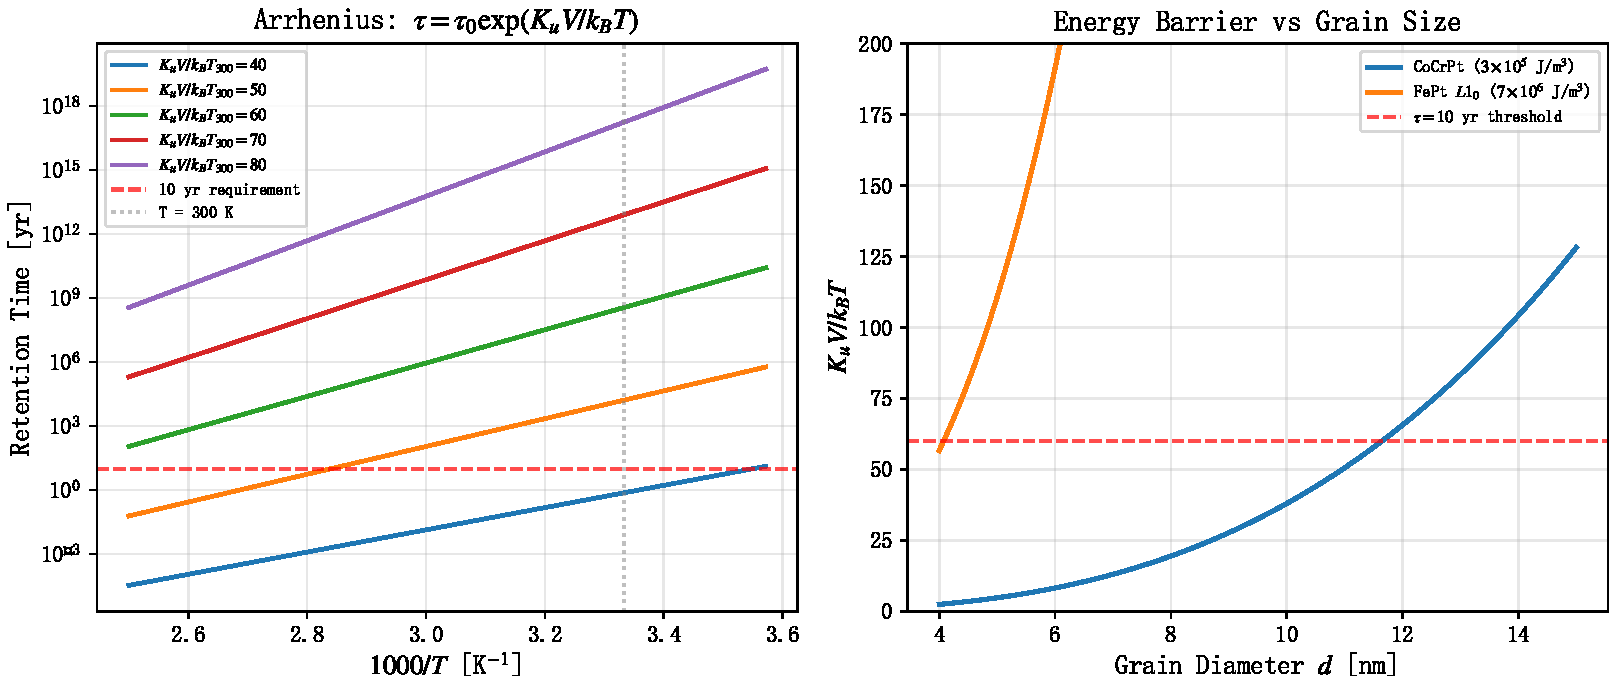
\includegraphics[width=0.85\textwidth]{fig-retention}
\caption{Arrhenius数据保持。
\textbf{左}：不同$K_u V/k_B T_{300}$值下，保持时间随温度的变化（对数纵轴）。
$K_u V/k_B T_{300} < 50$时，即使室温下保持时间也远低于10年要求。
\textbf{右}：对CoCrPt（$K_u \approx 3\times 10^5$ J/m$^3$）和
FePt $L1_0$（$K_u \approx 7\times 10^6$ J/m$^3$），
能垒$K_u V/k_B T$随晶粒直径的变化。水平虚线为$\tau = 10$年的判据（$K_u V/k_B T = 60$）。
CoCrPt的「生死线」约在$d \approx 8.5$ nm——当前1 Tb/in$^2$级介质的晶粒尺寸已逼近此极限。}
\label{fig:retention}
\end{figure}

对于有限外场$\mathbf{H}$沿易轴反方向作用的情况，能垒被降低。
修正的N\'{e}el-Brown公式为：
\begin{equation}
  \tau(H) = \tau_0 \exp\!\left[ \frac{K_u V}{k_B T}
            \left(1 - \frac{H}{H_K}\right)^n \right]
\end{equation}
其中$n = 2$（SW粒子，场严格沿易轴反方向）或$n \approx 1.5$（随机取向系综平均）。

\textbf{热辅助写入的本质}：即使$H < H_K$（在SW零温极限下不会翻转），
有限温度使翻转有一个非零的概率——热涨落「帮助」系统越过能垒。
翻转概率为$P_{\text{sw}} = 1 - \exp(-t_p/\tau(H))$。
这意味着写入是一个\textbf{随机过程}，永远无法达到$P_{\text{sw}} = 1$的确定性翻转。
写入错误率（WER）由$\tau(H)$、脉冲宽度$t_p$和温度$T$共同决定。

\section{写入：从感应写头到HAMR}

\subsection{Karlqvist场与单极写头}

写磁头是微米尺度的电磁铁。在准静态近似下，写场由静磁学Maxwell方程描述。
Karlqvist（1954）给出了二维缝隙场的解析解——垂直磁记录中写头正下方的
垂直场分量$H_z$近似为：
\begin{equation}\label{eq:karlqvist}
  H_z(x,z) = \frac{H_0}{\pi}\left[
    \arctan\!\left(\frac{x + g/2}{z}\right)
    - \arctan\!\left(\frac{x - g/2}{z}\right)
  \right]
\end{equation}
其中$g \approx 30$--$50$ nm为写间隙，$H_0 \approx NI/g$为间隙中心处的场强
（Amp\`{e}re定律），$z \approx 3$--$5$ nm为磁头飞行高度。

现代垂直磁记录采用\textbf{单极型写头}配合盘片下方的\textbf{软磁底层（SUL）}。
SUL（高磁导率薄膜，通常为NiFe或CoFe非晶合金）的镜像效应将单极子等效长度加倍，
大幅增强了记录层中的写场强度和均匀性。

\subsection{热辅助磁记录（HAMR）}
\label{sec:hamr}

HAMR是对三元悖论的首选工程解决方案。其物理思想简洁而深刻：
\begin{enumerate}
  \item 写入时，\textbf{局部加热}记录介质至$T_{\text{write}} \approx 600$--$700$ K
  （接近FePt $L1_0$的居里温度$T_C \approx 750$ K）。
  \item 在高温下，$M_s$下降（分子场理论给出$M_s(T) \propto (T_C - T)^{1/2}$
  在$T \to T_C$），各向异性$K_u$以更快的速率下降（$K_u(T) \propto M_s(T)^3$
  在单离子各向异性模型中）。因此$H_c$骤降——
  FePt在室温下$H_c \sim 70$ kOe，在$T_{\text{write}}$下仅$5$--$10$ kOe。
  \item 写磁头的中等磁场（$15$--$20$ kOe）在$T_{\text{write}}$下足以可靠翻转磁化方向。
  \item 冷却后（散热通过热传导至散热层，时间常数$\sim 100$ ps），
  介质恢复室温下的超高$H_c$——写入的磁化方向被「冻结」。」
\end{enumerate}

加热源是\textbf{近场光学换能器（NFT）}——一个Au等离子体纳米天线，
集成在写磁头滑块上。$\sim 830$ nm激光聚焦到NFT上后激发表面等离激元共振，
在尖端的曲率半径（$\sim 5$--$10$ nm）处产生极强的近场增强
（电场增强因子$\sim 10^3$--$10^4$），使加热光斑压缩至$\sim 20$--$30$ nm。

HAMR的使能材料是\textbf{$L1_0$有序FePt合金}。
FePt $L1_0$为四方晶系（$a = 3.85$ \AA, $c = 3.71$ \AA），
Fe和Pt原子沿c轴交替排列。其$K_u \approx 7 \times 10^6$ J/m$^3$的超高各向异性
来源于Fe-3d与Pt-5d的强自旋-轨道杂化——Pt的5d态具有巨大的SOC常数
（$\xi_{\text{Pt}} \approx 0.5$ eV，远高于Fe-3d的$\sim 0.05$ eV），
通过杂化将SOC「借给」了Fe的磁性电子。

\begin{physbox}
\textbf{HAMR的热物理并不简单。}写入过程中涉及多尺度热传导：
光斑（$\sim 25$ nm）内的光吸收$\to$ FePt层（$\sim 10$ nm厚）的电子-声子耦合
$\to$ 散热层的热扩散。面外热时间常数$\sim 100$ ps，
这就要求写场脉冲与激光脉冲的时间同步精度在$\pm 50$ ps以内。
同时，盘片高速旋转（$\sim 100$ m/s线速度）意味着
磁头下任一给定物理点在光斑内停留的时间仅$\sim 0.25$ ns——
HAMR的热-磁-力学耦合是当代信息存储中最精密的物理实验之一。
\end{physbox}

\section{读取：自旋极化输运与TMR}

\subsection{从GMR到TMR}

1990年代引入的巨磁阻（GMR）读头，以及2000年代中期升级的隧道磁阻（TMR）读头，
是自旋电子学最成功的商业应用。读取的物理挑战是：
\textbf{在不改变磁化状态的前提下，以亚纳米级分辨率检测$\sim 50$--$200$ Oe的
弱杂散磁场的方向。}

GMR效应的物理基础是Mott的双电流模型（1936）：在远低于$T_C$的温度下，
自旋翻转散射的速率远低于动量散射速率，自旋向上和自旋向下的传导电子可被视为
两个独立的并联导电通道。在铁磁金属中，两种自旋通道的电导率不同——
多数自旋电子经历较弱的s-d散射（因为d带末态密度较低），
少数自旋电子经历较强散射——自旋极化率$P = (\sigma_\uparrow - \sigma_\downarrow)/(\sigma_\uparrow + \sigma_\downarrow)$
（对Co, $P \approx 0.35$--$0.45$）。

\subsection{MgO(001)的Bloch态对称性筛选}

2004年的突破——MgO(001)单晶势垒实现TMR $> 600\%$——
揭示了一种完全不同于GMR态密度图像的物理机制：
\textbf{Bloch态对称性筛选}。

Butler等人（2001, PRB）的第一性原理Layer-KKR计算预言了这一效应。
物理图景如下：

\begin{enumerate}
  \item MgO的复能带结构中，在带隙内存在倏逝态。具有\textbf{$\Delta_1$对称性}
  （$k_\parallel = 0$点的全对称不可约表示，由$s$、$p_z$、$d_{3z^2-r^2}$轨道杂化构成）
  的倏逝态衰减常数最小（$\kappa_{\Delta_1} \approx 0.2$ \AA$^{-1}$），
  因此经MgO势垒传输的距离最长。

  \item bcc Fe（和CoFeB）的多数自旋能带中，在$E_F$处存在$\Delta_1$特征的Bloch态。
  少数自旋能带中，$E_F$处的Bloch态具有$\Delta_2$和$\Delta_5$对称性（由$d_{xz/yz}$等
  轨道杂化构成），\textbf{没有$\Delta_1$分量}。

  \item 因此：平行态中，$\Delta_1 \to \Delta_1 \to \Delta_1$的「高速公路」畅通——高透过率。
  反平行态中，$\Delta_1 \to \Delta_5$/$\Delta_2$的对称性失配使透过率指数级压制。
\end{enumerate}

\begin{figure}[htbp]
\centering
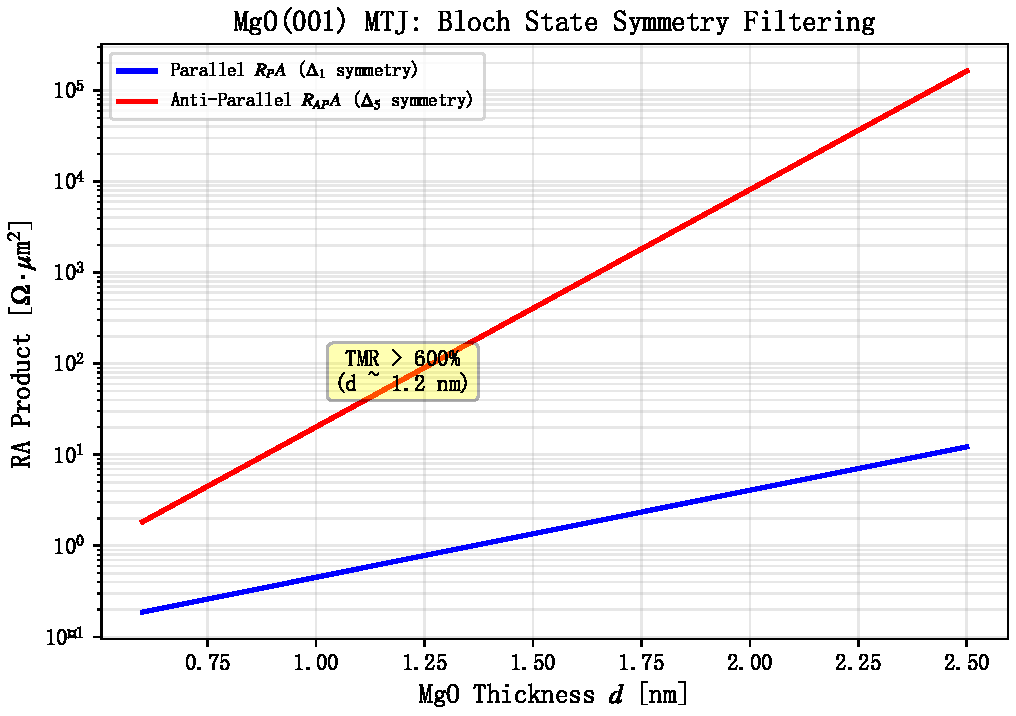
\includegraphics[width=0.7\textwidth]{fig-tmr-ra}
\caption{MgO(001) MTJ的RA积与MgO厚度的关系。
$\Delta_1$态（平行态）的低衰减常数$\approx 2.2$ nm$^{-1}$ vs
$\Delta_5$态（反平行态）的高衰减常数$\approx 6.0$ nm$^{-1}$，
使得两态的RA积以截然不同的斜率增长——在$d \approx 1.2$ nm附近，
TMR $> 600\%$变得可及。}
\label{fig:tmr}
\end{figure}

\subsection{读回信号链}

TMR读头的自由层磁化受介质杂散场$H_s$作用发生偏转。
读出电压信号为：$\Delta V \approx V_{\text{bias}} \times (\text{TMR}/2)(1 - \cos\theta)$，
小偏转角下$\Delta V \propto H_s$。信号幅度约$1$--$5$ mV。

主要噪声源（按贡献递减）：
\textbf{介质噪声}（晶粒尺寸/位置的随机性——主导，$\propto 1/\sqrt{N_{\text{grains}}}$）、
\textbf{Johnson热噪声}（$4k_B T R\Delta f$，$\sim 40$ $\mu$V rms）、
\textbf{磁噪声}（自由层热进动）、\textbf{散粒噪声}（$2eI\Delta f$，通常低于热噪声）。

HDD利用\textbf{低密度奇偶校验码（LDPC）}将原始BER从$\sim 10^{-3}$校正至
用户可见的$< 10^{-15}$。LDPC解码的「软判决」增益（约$2$--$3$ dB）来自
TMR读头提供的对数似然比（LLR）信息。

\section{介质微观结构与信号质量}

\subsection{晶粒系综的噪声}

垂直记录介质中的比特由$N \approx 10$--$20$个晶粒组成。
若各晶粒磁化方向独立且随机取向（仅受$K_u$和偶极耦合约束），
则比特的平均磁化方向存在统计涨落，涨落幅值$\propto 1/\sqrt{N}$。
随着面密度增加，$N$减小，介质噪声恶化——
这是记录密度的基本信噪比（SNR）瓶颈。

晶粒间的偶极耦合和残余交换耦合（通过晶界的间接耦合）导致
磁化翻转的集体行为——晶粒簇（cluster）的形成——在微磁学模拟中表现为
回线变斜（shearing）和翻转场的展宽（switching field distribution, SFD）。
Voronoi镶嵌的多晶微磁学模拟（Mumax$^3$, OOMMF）是定量评估这些效应的标准工具。

\subsection{从PMR到HAMR再到BPM}

密度演进的路线图清晰地反映了物理瓶颈的逐步突破：
\begin{itemize}
  \item \textbf{垂直磁记录（PMR）}（2005--至今）：$K_{\text{eff}} > 0$，
  晶粒尺寸$\sim 8$--$10$ nm，面密度$\sim 1$--$1.5$ Tb/in$^2$。已逼近CoCrPt的超顺磁极限。
  \item \textbf{热辅助磁记录（HAMR）}（2024--）：采用超高$K_u$的FePt $L1_0$介质，
  以加热瞬态降低$H_c$解决可写性。面密度目标$> 3$ Tb/in$^2$。
  \item \textbf{比特图案化介质（BPM）}（未来）：每个比特定义在一个独立的、
  光刻或自组装制备的孤立磁岛上，岛间非磁性填充。在物理上彻底消除晶粒间交换耦合
  和偶极耦合——每个比特只有一个「晶粒」（即整个岛）。面密度目标$> 5$ Tb/in$^2$。
\end{itemize}

% ===================================================================
% CHAPTER 3
% ===================================================================
\chapter{半导体电荷存储物理}
\label{ch:nand}

\section{从磁化到电荷}

第2章阐述的磁性存储依赖大量自旋的集体行为——每个比特由10--20个CoCrPt晶粒的
平均磁化方向编码。本章转向一种截然不同的物理量作为信息载体：
\textbf{被绝缘层完全包围的纳米导体（浮栅）中的电子数目}。

这一转变带来了三个根本性的物理差异：
\begin{enumerate}
  \item \textbf{写入机制}：磁记录用磁场（通过写磁头电磁铁产生），
  闪存用电场（通过FN量子隧穿注入/移除电子）。
  \item \textbf{擦除粒度}：磁记录可以原地覆写（直接覆盖同一物理位置的磁化方向），
  闪存\textbf{不能}——修改一个比特需要先擦除包含$10^5$--$10^6$个比特的整个块。
  这一物理事实直接催生了闪存转换层（FTL）和异地更新策略。
  \item \textbf{统计涨落的角色}：在磁记录中，每比特由10--20个晶粒的平均磁化编码，
  统计涨落被平均化。在闪存中，先进节点（QLC）的每状态仅有$\sim 20$--$30$个电子的差异——
  Poisson涨落直接决定了多级存储的物理极限。
\end{enumerate}

\section{浮栅晶体管的静电学}

\subsection{从MOSFET到浮栅晶体管}

浮栅晶体管（FGMOS）由Frohman-Bentchkowsky于1971年在Intel发明。
与标准n沟道MOSFET相比，FGMOS在控制栅（CG）与沟道之间插入了一个
\textbf{电学浮空的多晶硅导体（浮栅，FG）}，并在CG-FG之间增加了第二层
介质（块间介质层，IPD，通常为ONO叠层——氧化物-氮化物-氧化物）。

\begin{figure}[htbp]
\centering
\begin{tikzpicture}[scale=1.15]
  \fill[gray!20] (0,0) rectangle (9,5.5);
  \fill[blue!10] (0.5,0.5) rectangle (8.5,5.0);
  \node at (4.5,0.8) {p-Si 衬底 (掺杂 $N_A \approx 10^{17}$ cm$^{-3}$)};
  \fill[red!40] (1,1.8) rectangle (2.2,3.8); \node at (1.6,2.8) {n$^+$ 源极};
  \fill[red!40] (6.8,1.8) rectangle (8,3.8); \node at (7.4,2.8) {n$^+$ 漏极};
  \fill[yellow!70] (2.2,3.8) rectangle (6.8,4.15);
  \node at (4.5,3.97) {\footnotesize 隧穿氧化层 SiO$_2$ (5--7 nm)};
  \fill[orange!50] (2.8,4.15) rectangle (6.2,4.5);
  \node at (4.5,4.32) {\footnotesize 浮栅 FG (多晶Si)};
  \fill[purple!35] (2.8,4.5) rectangle (6.2,4.85);
  \node at (4.5,4.67) {\footnotesize IPD ONO (EOT 10--20 nm)};
  \fill[cyan!40] (2.8,4.85) rectangle (6.2,5.2);
  \node at (4.5,5.02) {\footnotesize 控制栅 CG (多晶Si/金属) = 字线};
  \draw[<->,thin] (2.4,4.15) -- (2.4,4.5) node[midway,left] {$C_{tun}$};
  \draw[<->,thin] (6.6,4.5) -- (6.6,4.85) node[midway,right] {$C_{IPD}$};
  \draw[<->,thin] (1.8,1.8) -- (1.8,3.8) node[midway,left] {沟道};
  \draw[|->,thin] (3.5,3.0) -- (5.5,3.0) node[midway,above] {$L \approx 20$--$50$ nm};
\end{tikzpicture}
\caption{浮栅晶体管（FGMOS）的层状结构。从底到顶：p-Si衬底上的n$^+$源/漏
$\to$ 隧穿氧化层 $\to$ 浮栅 $\to$ IPD（ONO叠层）$\to$ 控制栅（字线部分）。
两个关键电容$C_{tun}$和$C_{IPD}$构成一个电容分压网络。}
\label{fig:fgmos-structure}
\end{figure}

\subsection{电容耦合模型}

FGMOS的电路本质是一个电容分压网络。浮栅节点储存净电荷$Q_{FG}$
（当电子储存在浮栅中时，$Q_{FG} < 0$），浮栅电压$V_{FG}$由Kirchhoff电荷守恒确定：
\begin{equation}\label{eq:charge-conservation}
  Q_{FG} = C_{IPD}(V_{FG} - V_{CG})
  + C_{tun}(V_{FG} - V_{ch})
  + C_{src}(V_{FG} - V_S)
  + C_{drn}(V_{FG} - V_D)
  + C_{adj}(V_{FG} - V_{adj})
\end{equation}
定义总电容$C_{\text{total}} = C_{IPD} + C_{tun} + C_{src} + C_{drn} + C_{adj}$。

最重要的器件参数是\textbf{控制栅耦合比}：
\begin{equation}\label{eq:alpha-cg}
  \boxed{ \alpha_{CG} = \frac{C_{IPD}}{C_{\text{total}}} }
\end{equation}

$\alpha_{CG}$量度控制栅对浮栅电位的控制效率。典型值$0.50$--$0.65$，
取决于IPD与隧穿氧化层的厚度之比（IPD更厚$\to C_{IPD}$更小$\to \alpha_{CG}$更低）。
其他耦合比类似定义：$\alpha_{tun} = C_{tun}/C_{\text{total}}$等。

\subsection{阈值电压偏移——闪存器件工程的基石}

对于n沟道FGMOS，定义阈值电压$V_{th}$为沟道达到强反型（表面势
$\psi_s = 2\phi_F$）时所需的控制栅电压。在忽略衬底偏置效应的近似下，
由电容网络导出：
\begin{equation}\label{eq:vth-fg}
  \boxed{ V_{th} = V_{th0} + \frac{Q_{FG}}{C_{IPD}} }
\end{equation}
其中$V_{th0}$为浮栅无净电荷时的中性阈值电压：
\begin{equation}
  V_{th0} = V_{FB} + 2\phi_F + \frac{\sqrt{4\varepsilon_{Si}qN_A(2\phi_F)}}{C_{ox}},
  \quad \phi_F = \frac{k_B T}{q}\ln\frac{N_A}{n_i}
\end{equation}

\Cref{eq:vth-fg}的物理图像极其清晰：\textbf{浮栅中每注入一个电子，
阈值电压就上移一个固定量——「单电子电压」$\Delta V_{th}^{1e} = e / C_{IPD}$}。
这是闪存器件工程的基石公式。

\begin{physbox}
\textbf{单电子阈值的数值估算。}对于先进节点FGMOS：
浮栅面积$A_{FG} \approx 20 \times 20$ nm$^2 = 4 \times 10^{-16}$ m$^2$，
IPD等效氧化层厚度（EOT）$t_{IPD}^{\text{EOT}} \approx 12$ nm，
$C_{IPD} = \varepsilon_0\varepsilon_{SiO_2}A_{FG}/t_{IPD} \approx 1.2 \times 10^{-18}$ F。
单电子阈值偏移：$\Delta V_{th}^{1e} = e/C_{IPD} \approx 1.6\times 10^{-19} / 1.2\times 10^{-18} \approx 133$ mV。

\textbf{对QLC的致命约束。}对于QLC（16级），总阈值窗口$\approx 4$ V，
平均级间距$\approx 250$ mV。但电子注入/抽取是Poisson过程——
每个状态下的电子数涨落$\sigma_N = \sqrt{\bar{N}}$。
若$\bar{N} \approx 50$（QLC的最低编程态），则$\sigma_N \approx 7$个电子，
$\sigma_{V_{th}} \approx 7 \times 133 \approx 930$ mV——已远超级间距！
因此实际QLC必须大幅增大浮栅面积（减小$C_{IPD}$使单电子偏移减小）
和/或采用更精密的ISPP算法压缩分布宽度。
\end{physbox}

\section{Fowler-Nordheim量子隧穿}

\subsection{WKB推导}

当隧穿氧化层（SiO$_2$）两端的电场$E_{ox}$超过约$6 \times 10^8$ V/m时，
SiO$_2$导带发生能带弯曲，形成三角形势垒。来自n$^+$多晶硅（或沟道反型层）
的电子通过量子隧穿穿越该势垒——此即\textbf{Fowler-Nordheim隧穿}。

在WKB（Wentzel-Kramers-Brillouin）近似下，能量为$E_x$（纵向动能）的电子
隧穿通过一维势垒$V(x)$的概率为：
\begin{equation}\label{eq:wkb}
  T(E_x) = \exp\!\left[ -2\int_{x_1}^{x_2} \kappa(x)\,dx \right],\quad
  \kappa(x) = \sqrt{\frac{2m^*_{ox}}{\hbar^2}\bigl[V(x) - E_x\bigr]}
\end{equation}
其中$m^*_{ox} \approx 0.42\,m_e$为SiO$_2$中电子的有效质量，
$x_1, x_2$为经典转折点（$V(x) = E_x$）。

对于三角形势垒（能带图如图\ref{fig:fn-barrier}所示）：
$V(x) = \phi_B - eE_{ox}x$（$\phi_B \approx 3.15$ eV为Si/SiO$_2$导带偏移）。
经典转折点：$x_1 = 0$，$x_2 = (\phi_B - E_x)/(eE_{ox})$。
代入WKB积分：
\begin{equation}
  \int_0^{x_2} \sqrt{\phi_B - E_x - eE_{ox}x}\,dx
  = \frac{2(\phi_B - E_x)^{3/2}}{3eE_{ox}}
\end{equation}
因此：
\begin{equation}
  T(E_x) = \exp\!\left[ -\frac{4\sqrt{2m^*_{ox}}}{3e\hbar E_{ox}}
            (\phi_B - E_x)^{3/2} \right]
\end{equation}

\begin{figure}[htbp]
\centering
\begin{tikzpicture}[scale=1.2]
  \draw[->] (0,-0.5) -- (0,6.5) node[left] {$E$};
  \draw[->] (-0.5,0) -- (8,0) node[below] {$x$};
  \fill[blue!10] (-0.5,3) rectangle (0,4.5);
  \node[blue] at (-0.4,3.7) {Si CB};
  \draw[thick,red!70!black] (0,3) -- (5.5,0.5);
  \fill[red!5] (0,0.5) -- (0,3) -- (5.5,0.5) -- (5.5,0.5) -- (0,0.5);
  \draw[<->] (-0.4,3) -- (-0.4,4.5) node[midway,left] {$\phi_B$};
  \draw[->,very thick,blue!60] (0,3.5) to[bend left=15] (3,1.5);
  \node[blue!60] at (1.5,3.2) {$\kappa(x)$};
  \draw[dashed] (0,3.5) -- (2.5,1.8) node[below] {$x_2$};
  \node at (4.5,1) {$V(x) = \phi_B - eE_{ox}x$};
  \node[red!70!black] at (6,0.2) {SiO$_2$ CB};
  \draw[fill=red!25] (6,-0.3) -- (6,0) -- (8,0) -- (8,-0.3) -- cycle;
\end{tikzpicture}
\caption{Fowler-Nordheim隧穿的能带图。氧化层电场$E_{ox}$将SiO$_2$导带倾斜为三角形
势垒。来自Si导带的电子经过WKB三角形势垒积分给出的隧穿概率穿越氧化层。}
\label{fig:fn-barrier}
\end{figure}

对发射电极中所有能量电子积分（采用$T = 0$的Sommerfeld模型——
供给函数在Fermi球内为常数），得到总FN电流密度：
\begin{equation}\label{eq:fn-current}
  \boxed{ J_{FN} = A_{FN} E_{ox}^2 \exp\!\left( -\frac{B_{FN}}{E_{ox}} \right) }
\end{equation}
其中：
\begin{align}
  A_{FN} &= \frac{e^3 m_e}{8\pi h m^*_{ox}\phi_B} \approx 1.2 \times 10^{-6}\ \text{A/V}^2 \\
  B_{FN} &= \frac{4\sqrt{2m^*_{ox}}\,\phi_B^{3/2}}{3e\hbar}
           \approx 2.35 \times 10^{10}\ \text{V/m}
\end{align}

\begin{figure}[htbp]
\centering
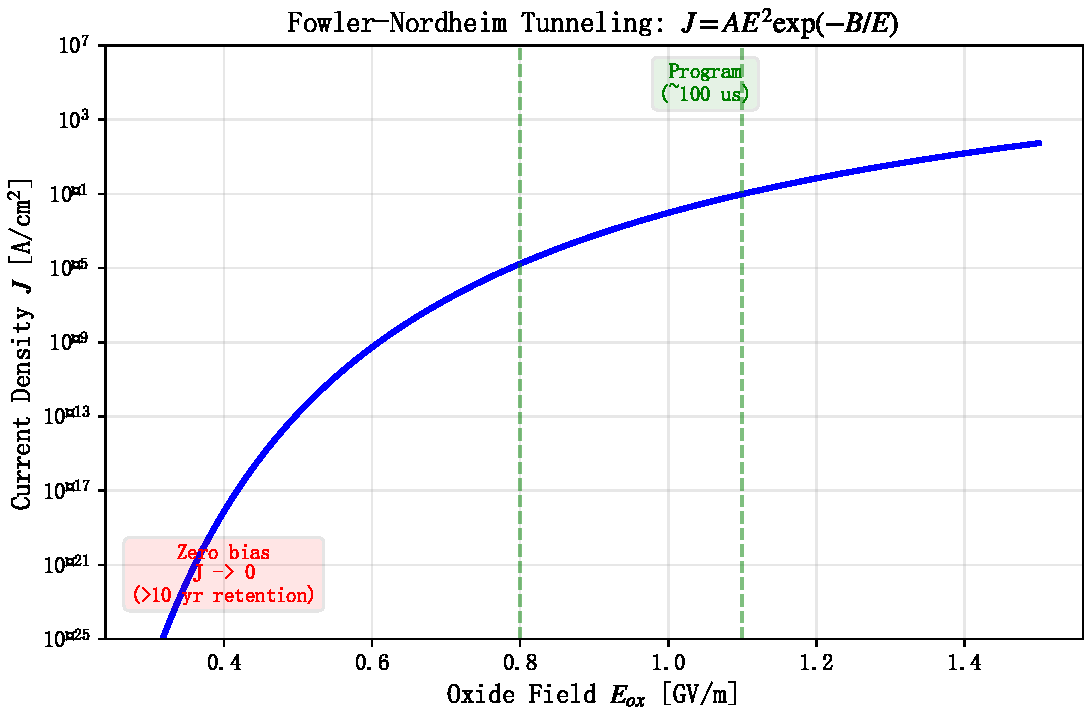
\includegraphics[width=0.7\textwidth]{fig-fn-tunneling}
\caption{Fowler-Nordheim隧穿的I-V特性。注意对数纵轴跨越25个数量级——
这是已知工程器件中最大的单机制电流动态范围（$\sim 10^{20}$倍）。
$E_{ox} \approx 1.1$ GV/m（编程）时电流$\sim 10^4$ A/cm$^2$；
零偏压下电流$< 10^{-20}$ A/cm$^2$——解释了同一器件何以同时实现
$\sim 100$ $\mu$s编程和$> 10$年数据保持。}
\label{fig:fn}
\end{figure}

\subsection{编程操作：ISPP算法}

编程时，控制栅加高压$V_{CG} \approx 15$--$20$ V，源/漏/衬底接地。
隧穿氧化层上电压$V_{ox} \approx \alpha_{CG} V_{CG}$，
$E_{ox} \approx 0.8$--$1.5 \times 10^9$ V/m。
电子从沟道反型层FN隧穿进入浮栅——这是自限过程：随浮栅电子积累，
$V_{FG}$下降$\to V_{ox}$减小$\to$隧穿电流衰减。

为精确控制编程后的阈值分布，实际采用\textbf{增量步进脉冲编程（ISPP）}：
\begin{enumerate}
  \item 施加编程脉冲（宽度$t_p \approx 10$--$30$ $\mu$s，幅度$V_{PGM}$）。
  \item 执行编程验证读取——判断$V_{th}$是否超过目标值$V_{th}^{\text{target}}$。
  \item 若未达目标：$V_{PGM} \leftarrow V_{PGM} + \Delta V_{PGM}$
  （步长$\Delta V_{PGM} \approx 0.2$--$0.5$ V），返回步骤1。
  \item 已达到目标：将该单元标记为「编程禁止」（通过自举偏置将沟道电位抬高，
  减小$V_{ox}$，有效抑制后续脉冲的FN隧穿）。
\end{enumerate}

ISPP确保最终阈值分布的标准差受$\Delta V_{PGM}$控制：
$\sigma_{V_{th}} \approx \alpha_{CG} \cdot \Delta V_{PGM} / 2$。

\section{多级存储：MLC/TLC/QLC的统计物理}

\subsection{阈值电压的分布模型}

在总阈值窗口约4 V内（0.5 V--4.5 V），$2^n$个状态被分配在优化的电压上。
第$k$个状态的$V_{th}$分布近似Gauss：
\begin{equation}\label{eq:vth-gauss}
  p_k(V) = \frac{1}{\sqrt{2\pi}\,\sigma_k}
           \exp\!\left[ -\frac{(V - \mu_k)^2}{2\sigma_k^2} \right]
\end{equation}
$\sigma_k$随$k$增大（更高$V_{th}$需要更多电子，注入涨落更大）。

\begin{figure}[htbp]
\centering
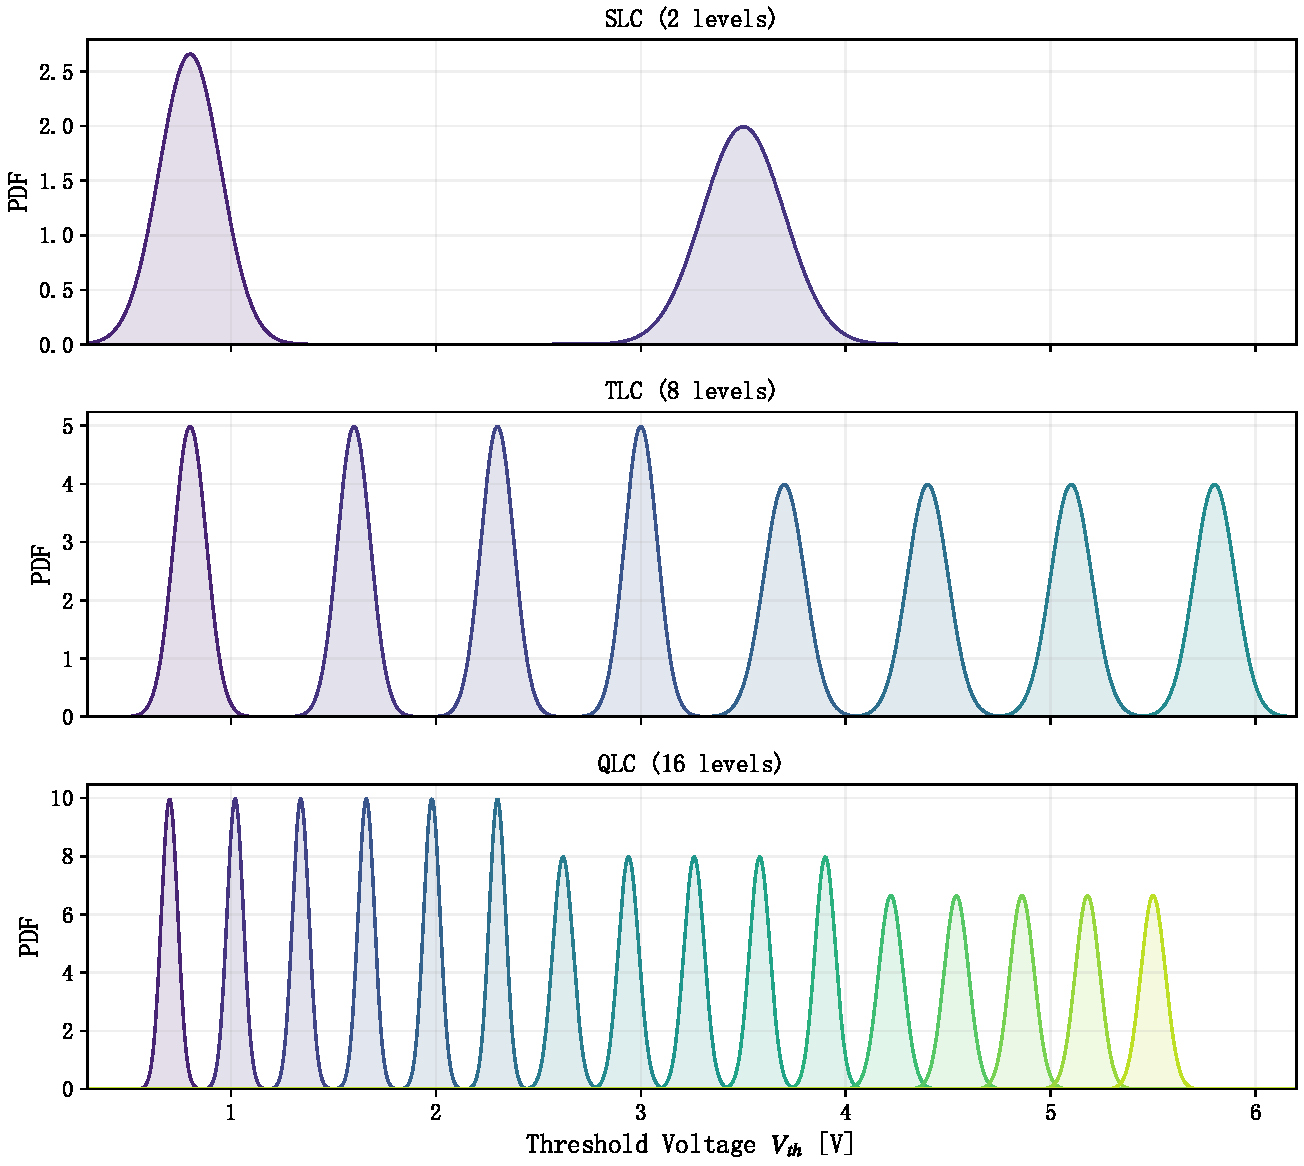
\includegraphics[width=0.9\textwidth]{fig-mlc-distributions}
\caption{SLC（2级）、TLC（8级）和QLC（16级）的阈值电压概率密度分布。
注意从TLC到QLC，分布尾部的交叠（overlap）急剧恶化——
这是多级闪存的根本物理瓶颈。}
\label{fig:mlc}
\end{figure}

\subsection{原始误码率的积分表达式}

相邻状态$k$与$k+1$之间的最优判决阈值（等先验概率下）为两Gauss分布的交点。
当$\sigma_k = \sigma_{k+1} = \sigma$时简化为中点：
$V_{\text{opt}} = (\mu_k + \mu_{k+1})/2$。

原始位错误率（Raw BER）由Gauss尾部的交叠积分给出：
\begin{equation}\label{eq:raw-ber}
  \boxed{ \text{BER}_{\text{raw}} = \frac{1}{2}\operatorname{erfc}\!\left(
    \frac{\Delta V}{2\sqrt{2}\,\sigma} \right) }
\end{equation}
其中$\Delta V = \mu_{k+1} - \mu_k$为级间距，
$\operatorname{erfc}(x) = (2/\sqrt{\pi})\int_x^\infty e^{-t^2}dt$。

典型TLC：$\Delta V \approx 400$ mV，$\sigma \approx 60$ mV
$\to \text{BER}_{\text{raw}} \approx 4.2 \times 10^{-4}$。
这必须通过LDPC/BCH纠错码校正至用户不可见的$< 10^{-15}$。
编码开销约为$7\%$--$15\%$（即闪存物理容量的$7\%$--$15\%$被ECC冗余占用）。

\begin{figure}[htbp]
\centering
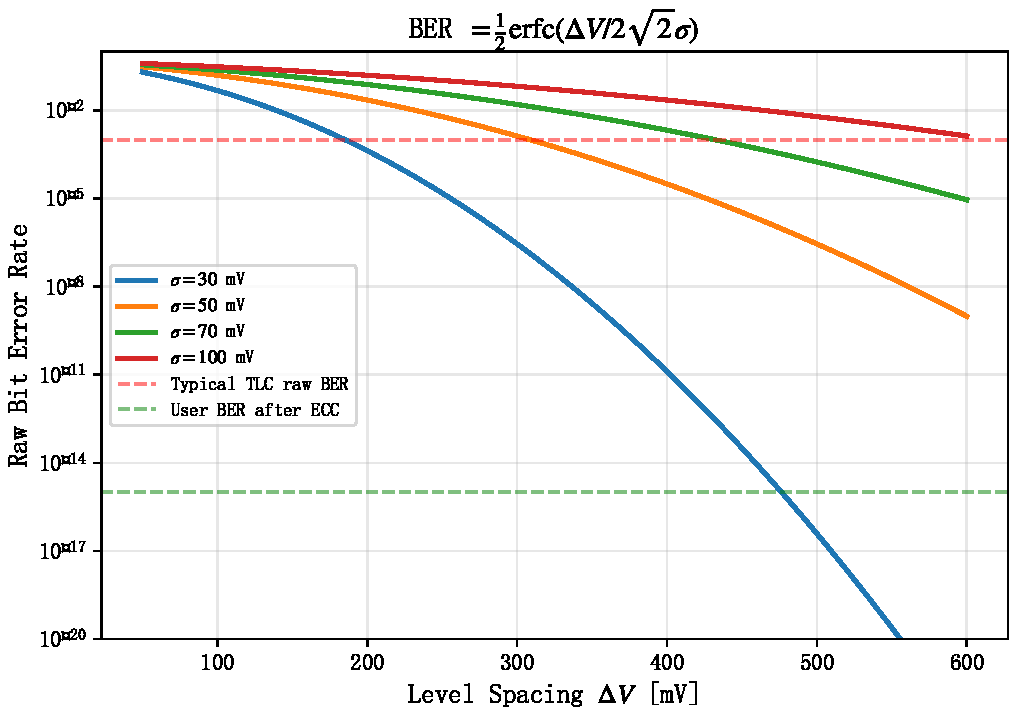
\includegraphics[width=0.65\textwidth]{fig-raw-ber}
\caption{原始BER随级间距$\Delta V$的变化，各曲线对应不同$\sigma$。
TLC的典型工作点（$\Delta V \approx 400$ mV, $\sigma \approx 60$ mV）对应的
raw BER $\approx 4\times 10^{-4}$。ECC（LDPC + BCH）将其校正至$< 10^{-15}$。}
\label{fig:ber}
\end{figure}

\subsection{Poisson涨落：QLC的终极物理约束}

对于QLC（16级），级间距仅$150$--$250$ mV。从\cref{eq:vth-fg}，
每个状态下的电子数差$\Delta N = C_{IPD}\Delta V/e$。
若$\Delta V = 200$ mV，则$\Delta N \approx 200/133 \approx 1.5$个电子——
这几乎不可行：Poisson涨落$\sigma_N = \sqrt{\bar{N}}$本身就超过相邻状态的电子数差！

实际QLC通过增大浮栅面积来降低单电子阈值偏移（$C_{IPD}$增大$\to \Delta V_{th}^{1e}$减小），
但代价是单元面积增大，密度优势被削弱。这是\textbf{电子离散性}这一量子力学事实
对闪存密度提升的根本约束——无论工艺如何进步，Poisson统计是绕不开的物理定律。

\section{隧穿氧化层的退化与可靠性}

\subsection{陷阱产生的微观机制}

每次P/E循环中，FN隧穿的高能电子（在$V_{ox} \approx 15$ V下，
电子穿越SiO$_2$导带底部时的功能可达$5$--$8$ eV）会打断Si-O键，
产生氧化层体陷阱和Si/SiO$_2$界面态。

主要退化机制：
\begin{itemize}
  \item \textbf{Si-H键断裂}：沟道界面处钝化Si-H键被高能电子打断，
  产生Si悬挂键（$P_b$中心）和自由H原子。H可扩散至氧化层内部，
  H$^+$在电场下漂移形成空间电荷。
  \item \textbf{氧空位生成}：SiO$_2$网格中O原子受撞击移位，
  产生$E'$中心（$\equiv$Si$\bullet$ Si$\equiv$，氧空位俘获一个电子）。
\end{itemize}

陷阱产生率与注入电荷总量$Q_{inj}$呈幂律关系：
$\Delta N_{it} \propto Q_{inj}^n$，$n \approx 0.4$--$0.6$。

\subsection{应力诱导漏电流（SILC）}

氧化层陷阱为电子提供了除直接FN隧穿之外的额外泄漏路径——
\textbf{陷阱辅助隧穿（TAT）}：电子以陷阱为「跳板」，分步穿过氧化层。
TAT电流正比于陷阱密度：
\begin{equation}
  J_{TAT} \propto N_{trap} \exp\!\left(
    -\frac{8\pi\sqrt{2m^*_{ox}}}{3hE_{ox}}\phi_t^{3/2} \right)
\end{equation}
其中$\phi_t$为陷阱能级深度。

SILC使得编程后浮栅中的电子缓慢泄漏——编程态$V_{th}$随时间下漂。
这是闪存数据保持退化的主要物理机制。

\begin{figure}[htbp]
\centering
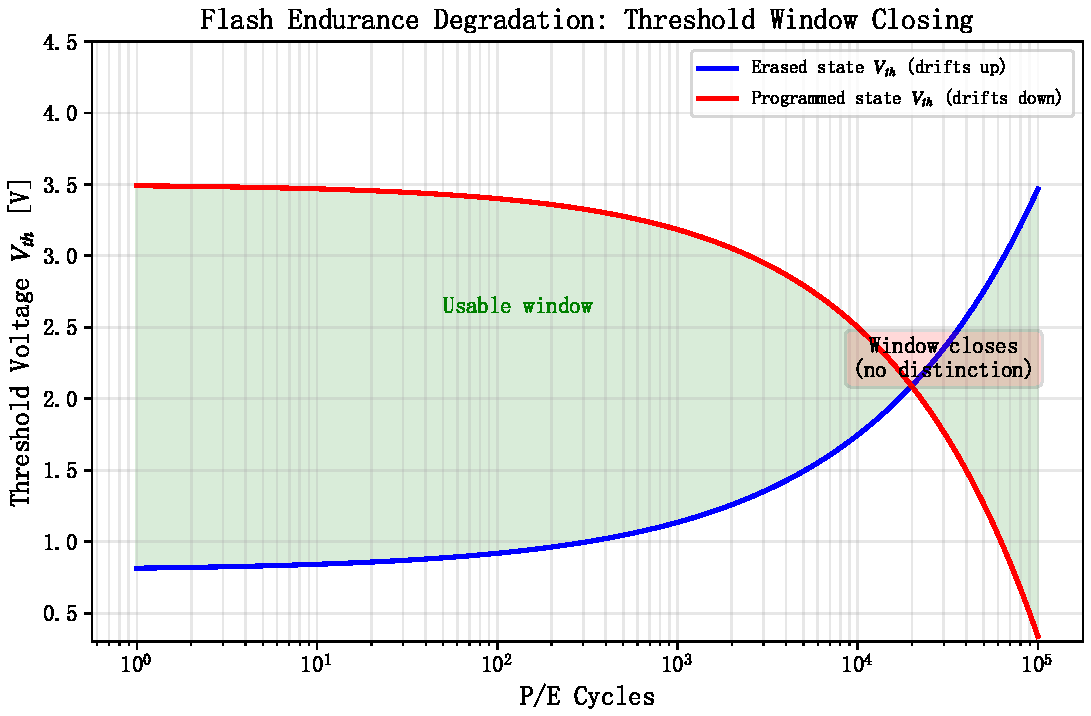
\includegraphics[width=0.7\textwidth]{fig-endurance}
\caption{闪存耐久性退化：阈值窗口随P/E循环的关闭。
擦除态$V_{th}$上漂（陷阱电荷屏蔽擦除电场），
编程态$V_{th}$下漂（SILC泄漏）。
当两态分布发生交叠时——该块不再可用。
SLC可承受$\sim 10^5$--$10^6$次P/E，TLC约$10^3$--$3 \times 10^3$次，
QLC低至$500$--$1000$次。}
\label{fig:endurance}
\end{figure}

\subsection{随机电报噪声（RTN）}

当单个氧化层陷阱恰好位于沟道界面附近时，该陷阱对电子的捕获/释放
随机切换（Poisson过程），导致$V_{th}$在离散的两水平间随机跳变——
即\textbf{随机电报噪声}。RTN导致的$V_{th}$跳变幅度近似为：
\begin{equation}
  \Delta V_{th}^{RTN} \approx \frac{e}{WL\,C_{ox}}
\end{equation}
对于$W \times L = 20 \times 20$ nm$^2$的单元，$C_{ox} \approx 2.5 \times 10^{-17}$ F，
$\Delta V_{th}^{RTN} \approx 6$ mV——对SLC和MLC可忽略，
但对QLC（级间距$\sim 150$ mV），这是读取窗口预算的重要组成部分。

\subsection{Arrhenius数据保持}

保持时间的温度依赖：
\begin{equation}
  t_{\text{ret}}(T) = t_{\text{ret}}(T_0)\exp\!\left[
    \frac{E_a}{k_B}\!\left(\frac{1}{T} - \frac{1}{T_0}\right)
  \right]
\end{equation}
激活能$E_a \approx 1.0$--$1.2$ eV。
在室温附近$E_a/k_B \approx 1.16 \times 10^4$ K：
\textbf{温度每升高约5$^\circ$C，保持时间约减半}。
这是SSD工作温度上限（通常70$^\circ$C）和「冷存储」概念的物理根源。

\section{阵列组织与闪存转换层}

\subsection{NAND串与块擦除}

NAND闪存的基本阵列单元是\textbf{NAND串}：64--128个FGMOS串联连接，
两端通过选择晶体管（SSL/DSL）连接到位线和源线。串联架构大幅减少了接触孔数量，
提高了存储密度。读取时，未选中字线接通过电压$V_{pass} \approx 5$--$6$ V
强制导通（工作在线性区），选中字线接读电压$V_{ref}$。

NAND闪存的\textbf{擦除以块（Block）为单位}（通常64--512页，每页16 KB）。
物理原因：所有单元的p阱共享同一衬底接触——擦除时需对整个p阱加高压
$V_{ERS} \approx 15$--$20$ V（控制栅接地），无法仅擦除单个单元。
这一事实直接导致了NAND闪存\textbf{不能原地覆写}的根本物理限制。

\subsection{3D NAND：从浮栅到电荷陷阱}

2013年后，NAND从平面走向垂直堆叠（3D NAND），当前已超过300层。
关键技术转变是用\textbf{电荷陷阱氮化硅（Si$_3$N$_4$）}替代多晶硅浮栅。

Si$_3$N$_4$中电荷被离散深能级陷阱捕获（陷阱密度$\sim 10^{19}$ cm$^{-3}$，
能级深度$\sim 1.0$--$1.5$ eV），而非均匀分布在浮栅中。
物理优势：
\begin{itemize}
  \item 电荷局域化——单元间电容耦合干扰（CCI）被抑制。
  \item 更薄的存储层（$\sim 5$ nm vs $\sim 10$ nm浮栅），适合垂直堆叠。
  \item 陷阱间相互隔离——单个陷阱的泄漏不影响邻近陷阱。
\end{itemize}

3D NAND的电荷注入机制仍是FN隧穿，但注入Si$_3$N$_4$层后通过
\textbf{Poole-Frenkel（PF）发射}在陷阱间跃迁分布。
PF电流为$J \propto E\exp[-(e/k_B T)(\phi_t - \sqrt{eE/\pi\varepsilon})]$，
物理图像为陷阱势垒在电场下的库仑势降低。

\subsection{FTL：物理限制的工程响应}

闪存转换层（FTL）是SSD控制器固件的核心，维护逻辑块地址（LBA）
到物理页地址（PPA）的动态映射。当主机「覆写「LBA $X$时：
物理流程为：分配新空闲页$P_{\text{new}}$ $\to$ 写入新数据 $\to$
旧页$P_{\text{old}}$标记为「无效（stale）」 $\to$ 更新映射表。
\textbf{旧页$P_{\text{old}}$的浮栅电荷完好无损}——数据物理保留至垃圾回收
（GC）擦除该块。GC的时机取决于写入模式和空闲空间份额，
从秒到永不——这正是第6章讨论的数据残留的物理基础。

% ===================================================================
% CHAPTER 4
% ===================================================================
\chapter{光子存储物理}
\label{ch:optical}

\section{光子替代电子与自旋}

前两章分别讨论了基于磁性和电荷的存储机制——它们合计贡献了全球数据存储容量的
约95\%。本章转向第三种物理机制：\textbf{光子与物质的相互作用}——即光学存储。

光学存储与磁性/电荷存储的根本区别在于：信息以介质表面或体内的反射率、偏振态
或折射率的空间调制来编码，而写入和读取的「探针」是聚焦的激光束而非磁头或
隧道电流。这赋予了光学存储一项独特的物理特性：\textbf{介质与读取设备物理分离}——
盘片可自由取出/放入驱动器（与此对比，HDD盘片和磁头被密封在氦气环境中，
SSD的NAND芯片永久焊在PCB上）。

\section{衍射极限：面密度的光学天花板}

光学存储的面密度受衍射极限的严格约束——这是远场光学的基本定律。
在标量衍射理论中（NA $< 0.6$），聚焦光斑的强度分布由Airy函数给出：
\begin{equation}\label{eq:airy}
  I(r) = I_0 \left[ \frac{2 J_1(k r\sin\alpha)}{k r\sin\alpha} \right]^2
\end{equation}
第一暗环半径——即Rayleigh分辨判据：
\begin{equation}
  r_0 = \frac{0.61\lambda}{\sin\alpha} = \frac{0.61\lambda}{\text{NA}}
\end{equation}

光学存储的密度进化史本质上就是光学的波长-NA进化史：

\begin{table}[H]
\centering
\caption{三代光盘技术的物理演进}
\begin{tabular}{@{}lccccccc@{}}
\toprule
格式 & 年代 & $\lambda$ [nm] & NA & 光斑直径 [$\mu$m] & 道间距 [nm] & 最短标记 [nm] & 单层容量 \\
\midrule
CD   & 1982 & 780 (近红外) & 0.45 & 2.1  & 1600 & 830  & \SI{700}{MB} \\
DVD  & 1996 & 650 (红光)   & 0.60 & 1.3  & 740  & 400  & \SI{4.7}{GB} \\
BD   & 2006 & 405 (蓝紫光) & 0.85 & 0.58 & 320  & 150  & \SI{25}{GB} \\
\bottomrule
\end{tabular}
\end{table}

\begin{figure}[htbp]
\centering
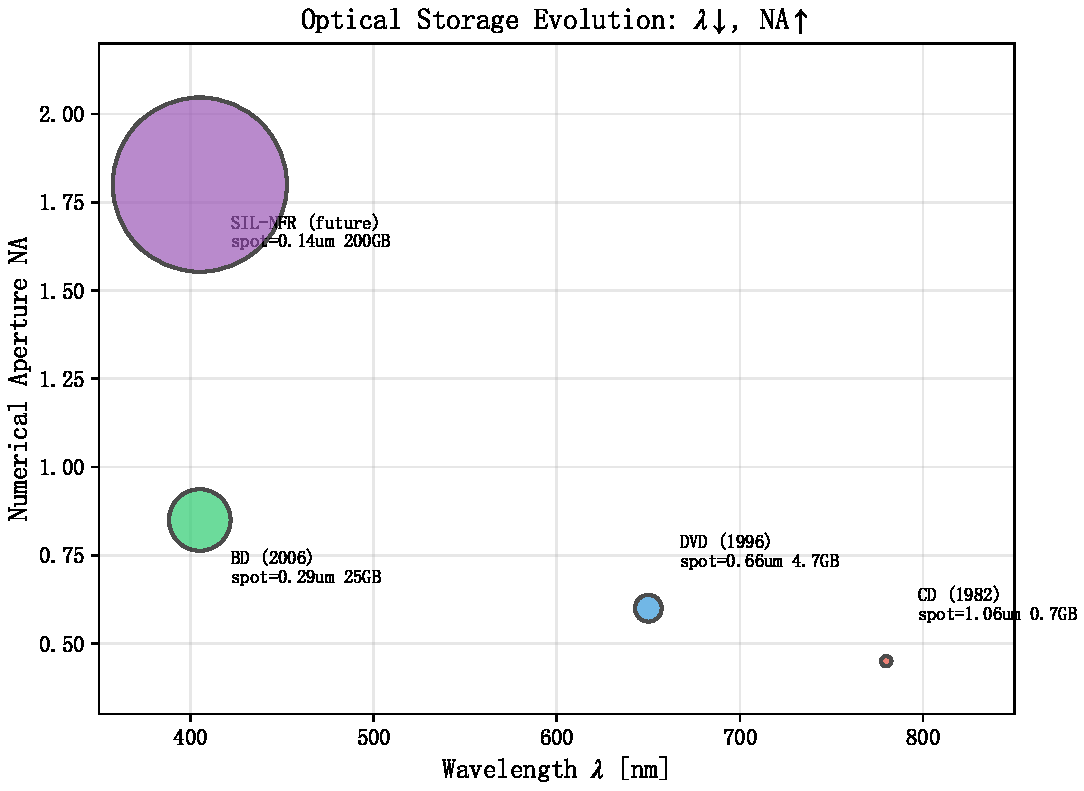
\includegraphics[width=0.7\textwidth]{fig-optical-evolution}
\caption{光盘技术的波长-NA演化。气泡面积正比于单层容量。
趋势明确：$\lambda \downarrow$，NA $\uparrow$，光斑$\downarrow$，容量$\uparrow$。
SIL-NFR（固体浸没透镜近场记录，紫色）展望了远超自由空间衍射极限的未来。}
\label{fig:optical-evolution}
\end{figure}

\subsection{矢量衍射理论：Richards-Wolf Debye积分}

当NA $> 0.6$时，光的矢量性质（偏振和纵向场分量）不可忽略。
Richards \& Wolf（1959）建立了高NA聚焦的矢量Debye理论——
焦点附近的电场由光瞳函数$\mathbf{E}_\infty(\theta,\phi)$的球面波角谱积分给出：
\begin{equation}\label{eq:debye}
  \mathbf{E}(\mathbf{r}) = -\frac{ikf}{2\pi}
  \iint_\Omega \mathbf{E}_\infty(\theta,\phi)\,
  e^{ik\hat{\mathbf{s}}\cdot\mathbf{r}}\,d\Omega
\end{equation}

对于沿$x$方向偏振的入射光，焦点附近电场可分解为Debye衍射积分$I_{0,1,2}$的组合。
关键的发现是：\textbf{在高NA下，$E_z$分量（沿光轴的纵向场）不可忽略}——
当NA $= 0.85$时，焦斑中心$|E_z|^2$占比可超过总强度的30\%。
纵向场的存在导致聚焦光斑沿偏振方向（$x$方向）拉伸为椭圆形——
这是在Blu-ray等近场高NA系统中必须考虑的效应。

\subsection{近场光学与固体浸没透镜}

衍射极限不是绝对不可突破——它所限制的是远场聚焦。
\textbf{近场光学}利用倏逝波（evanescent wave）可实现亚波长场局域。
倏逝波的横向波矢$k_\parallel > k$（自由空间波数），
法向波矢为纯虚数$k_z = i\sqrt{k_\parallel^2 - k^2}$，
场沿法线指数衰减$\propto \exp(-|k_z|z)$。

\textbf{固体浸没透镜（SIL）}是实现近场记录的核心方案。
SIL由高折射率材料（GaP, $n \approx 3.3$--$3.5$）制成，
置于盘片与物镜之间。利用折射率失配激发倏逝波，
有效NA为$\text{NA}_{\text{eff}} = n_{\text{SIL}}\times \text{NA}_{\text{obj}}$（半球形），
或$\text{NA}_{\text{eff}} = n_{\text{SIL}}^2\times \text{NA}_{\text{obj}}$（超半球/aplanatic）。
对于$n_{\text{SIL}} \approx 3.4$、NA$_{\text{obj}} \approx 0.8$的半球形SIL，
$\text{NA}_{\text{eff}} \approx 2.7$——远超过$1.0$的自由空间极限！
SIL与盘片的间距需控制在$< 25$ nm（亚纳米级气浮定位精度），
可在$\lambda = 405$ nm下实现$\sim 100$ nm的聚焦光斑。

\section{相变存储介质：GST的非晶-晶态切换}

\subsection{GST-225的材料物理}

可擦写光盘的记录层为硫系相变合金，最典型的配方是
\textbf{Ge$_2$Sb$_2$Te$_5$}（GST-225）及其掺杂变体。
硫系玻璃的特征是在非晶态和晶态之间具有巨大的光学（和电学）对比度。

GST-225的稳态晶相为亚稳态NaCl型立方结构（$Fm\bar{3}m$空间群，
$a = 6.0$ \AA），Te原子占据4a位（一个fcc子晶格），
Ge和Sb原子随机占据4b位（另一个fcc子晶格），并伴随约20\%的结构空位。
非晶态则长程无序。

两态间的反射率对比来源于复折射率$n + i\kappa$的差异——
在405 nm处：非晶态$(4.2 + i0.3)$ vs 晶态$(1.7 + i3.0)$。
消光系数$\kappa$的大幅增加（$\to$更高反射率）源于晶态中电子态的离域化：
能带填充，带隙从非晶态的$\sim 0.7$ eV减小到晶态的$\sim 0.5$ eV。

\subsection{写入：熔化-淬冷非晶化}

写入（「刻录」非晶标记）的核心物理是\textbf{超快激光加热-熔化-急冷循环}：
\begin{enumerate}
  \item 激光脉冲（功率10--20 mW，脉宽10--100 ns）聚焦至$\sim 0.5$ $\mu$m直径
  区域，功率密度$\sim 10^7$--$10^8$ W/cm$^2$。
  \item GST温度在几纳秒内超过$T_m \approx 610$--$630^\circ$C——熔化。
  液态中原子充分扩散，原有晶序被完全摧毁。
  \item 激光结束后，热量通过热传导迅速扩散至介质多层膜（ZnS-SiO$_2$保护层 +
  Ag反射层）。淬冷速率$dT/dt \sim 10^9$--$10^{10}$ K/s，
  远超GST-225的临界冷却速率（$\sim 10^8$ K/s），
  熔融态被「冻结」在无序的非晶态。
\end{enumerate}

\subsection{擦除：固相晶化的JMAK动力学}

擦除操作将非晶标记恢复到晶态——需要将其加热至
$T_g$（玻璃转变温度，$\sim 150^\circ$C）以上、$T_m$（熔点）以下的温度窗口。
在此窗口内，成核（nucleation）和生长（growth）共同驱动非晶$\to$晶转变。

经典成核理论（CNT）给出稳态成核率：
\begin{equation}
  I_{ss} = N_0\frac{k_B T}{h}\exp\!\left( -\frac{\Delta G_c + E_a}{k_B T} \right),\quad
  \Delta G_c = \frac{16\pi}{3}\frac{\sigma^3}{(\Delta G_V)^2}
\end{equation}
其中$\Delta G_V = \Delta H_f \Delta T / T_m$为体自由能驱动力，$E_a$为原子跨界面输运的扩散激活能
（$\Delta T = T_m - T$为过冷度），$\sigma$为晶/非晶界面自由能。

晶化体积分数的时间演化由
\textbf{Johnson-Mehl-Avrami-Kolmogorov（JMAK）方程}描述：
\begin{equation}\label{eq:jmak}
  \boxed{ \chi(t) = 1 - \exp\!\bigl[ -k(T)\,t^n \bigr] }
\end{equation}
Avrami指数$n$取决于成核和生长的维度：
$n \approx 3$--$4$对应持续成核+三维生长，
$n \approx 1$--$2$对应预存核+低维生长。

生长速率$u(T)$（Turnbull表达式）在$\sim 450$--$500^\circ$C达到峰值
$\sim 1$ m/s——这比典型的硅酸盐玻璃晶化速度快5--6个数量级，
是GST作为相变存储材料的核心优势之一。

\subsection{可擦写循环的失效}

反复写/擦导致相变材料的退化：
\begin{itemize}
  \item \textbf{偏析}：Te富集相的形成改变了局部化学计量比。
  \item \textbf{空洞形成}：反复熔化/淬冷引入的应力在GST层中成核微空洞，
  降低光学对比度。
  \item \textbf{界面互扩散}：GST与保护层（ZnS-SiO$_2$）之间的原子互扩散
  降低了多层膜的光学干涉对比度。
\end{itemize}
典型可擦写光盘的循环次数约$1000$--$10000$次——
远低于磁光记录（$> 10^6$），这是相变存储的核心可靠性弱点。

\section{磁光记录与全息存储}

\subsection{磁光Kerr效应的介电张量描述}

磁光记录利用磁性材料的\textbf{极向Kerr效应（MOKE）}进行读取。
当线偏振光从磁化介质表面反射时，偏振面发生旋转——旋转角$\theta_K \propto M_z$。
在宏观电动力学中，MOKE来源于介电张量中的反对称非对角元：
\begin{equation}
  \boldsymbol{\varepsilon} =
  \begin{pmatrix}
    \varepsilon_{xx} & \varepsilon_{xy} & 0 \\
    -\varepsilon_{xy} & \varepsilon_{xx} & 0 \\
    0 & 0 & \varepsilon_{zz}
  \end{pmatrix},\quad
  \varepsilon_{xy} \propto iQM_z
\end{equation}
磁光介质的本征模为左旋和右旋圆偏振光（具有不同的折射率$n_\pm$），
Kerr旋转角为$\Phi_K = i\varepsilon_{xy}[\sqrt{\varepsilon_{xx}}(\varepsilon_{xx} - 1)]^{-1}$。

写入采用\textbf{热磁写入}：亚铁磁TbFeCo薄膜具有补偿温度$T_{\text{comp}}$，
在此温度附近$H_c \to \infty$（因$M_s \to 0$），
而在更高温度（$\sim 200$--$300^\circ$C）处$H_c$骤降至
$\sim 100$--$300$ Oe——可被外置永磁体翻转。

\subsection{全息体存储：从面到体}

全息存储将信息以\textbf{体Bragg光栅}形式记录在光折变晶体
（如LiNbO$_3$:Fe，铌酸锂掺铁）中——这是从二维面存储到三维体存储的范式转换。

信号光（携带SLM页面数据）与参考光相交产生干涉条纹：
$I(\mathbf{r}) = I_S + I_R + 2\sqrt{I_S I_R}\cos(\mathbf{K}\cdot\mathbf{r})$，
光栅矢量$\mathbf{K} = \mathbf{k}_S - \mathbf{k}_R$。
光强亮区激发深能级Fe$^{2+}$电子至导带$\to$扩散/漂移重新分布
$\to$被Fe$^{3+}$深陷阱捕获$\to$产生空间电荷场$E_{sc}$
$\to$通过线性Pockels效应$\Delta n = -\frac12 n_0^3 r_{\text{eff}} E_{sc}$
调制折射率。

读回时满足Bragg条件$2\Lambda\sin\theta_B = \lambda$的参考光衍射重建信号光。
角度复用的选择性$\Delta\theta_{1/2} \approx \lambda/(d\sin\theta_B)$
（$d$为晶体厚度，对于1 cm LiNbO$_3$约为$0.003^\circ$）使同一晶体可存储数千页。

% ===================================================================
% CHAPTER 5
% ===================================================================
\chapter{新物理·新存储}
\label{ch:emerging}

\section{超越磁滞与浮栅}

前三章建立了三种经典存储技术的物理框架。这些技术正在逼近其物理缩放极限：
HDD遭遇超顺磁极限（$K_u V/k_B T > 60$，第2章）；
NAND闪存面临隧穿氧化层厚度不可再降（直接隧穿泄漏）和电子离散性
（QLC的$\sim 20$--$30$电子/状态差异）的双重瓶颈（第3章）。
光学存储受远场衍射极限的约束（第4章）。

本章聚焦四种「后传统」时代的新型存储技术。它们的共同特征是：
采用\textbf{不同于磁滞和浮栅电荷的物理量}作为信息载体，
从而在根本上绕开传统技术的缩放瓶颈。
这四类技术分别从凝聚态物理的四个分支汲取灵感：
自旋电子学（STT/SOT-MRAM）、缺陷化学与离子输运（ReRAM）、
相变动力学（PCM）和铁电体物理（FeFET）。

\section{自旋转移矩MRAM（STT-MRAM）}

\subsection{从磁场写入到电流写入}

传统MRAM使用外加磁场（通过导线电流的Oersted场）翻转自由层磁化——
需要$\sim 10$ mA的写入电流和较大单元面积（导线产生的场随距离衰减）。
第2章讨论的HDD写磁头也依赖外磁场——但那是通过微米级电磁铁产生的。
STT-MRAM的革命性在于：\textbf{完全抛弃外磁场写入，改用自旋极化电流
直接翻转磁化}。

写入机制的核心物理是\textbf{自旋转移矩（STT）}——由Slonczewski和Berger
在1996年独立预言。当电流穿过磁化固定的参考层（RL，充当自旋极化器）后，
传导电子携带了沿RL磁化方向$\hat{\mathbf{p}}$的自旋角动量。
这些自旋极化电子进入自由层（FL）后，其横向自旋分量通过s-d交换作用传递给FL的
局域磁矩。由角动量守恒，这等效于在FL磁化$\mathbf{m}$上施加了
\textbf{自旋转移力矩}。

\subsection{LLG-Slonczewski方程与临界电流}

包含STT的广义LLG方程——\textbf{LLG-Slonczewski方程}：
\begin{equation}\label{eq:llg-stt}
  \boxed{
  \frac{\partial\mathbf{m}}{\partial t}
  = -\gamma\mathbf{m}\times\mathbf{H}_{\text{eff}}
  + \alpha\mathbf{m}\times\frac{\partial\mathbf{m}}{\partial t}
  + \frac{\gamma\hbar I}{2e M_s V}\,g(\theta)\,
    \mathbf{m}\times(\mathbf{m}\times\hat{\mathbf{p}})
  }
\end{equation}
其中$g(\theta) = [-4 + (1+P)^{3/2}(3+\cos\theta)/(4P^{3/2})]^{-1}$为Slonczewski自旋转移效率因子，
$\theta$为$\mathbf{m}$与$\hat{\mathbf{p}}$的夹角。

\textbf{STT项的数学形式$(\mathbf{m}\times(\mathbf{m}\times\hat{\mathbf{p}}))$
与阻尼项相同}——这意味着STT可视作\textbf{电流诱导的正/负阻尼}。
当STT方向与自然Gilbert阻尼相反的幅度超过自然阻尼时，
磁化获得净能量，可被驱动翻转到另一个稳定方向。

在$\alpha \ll 1$极限下，线性稳定性分析给出零温临界电流：
\begin{equation}\label{eq:Ic0}
  \boxed{ I_{c0} = \frac{2e}{\hbar}\frac{\alpha}{g(0)}\,E_b
  = \frac{2e}{\hbar}\frac{\alpha}{g(0)}\,K_u V }
\end{equation}

\textbf{标度}：$I_{c0} \propto \alpha K_u V$。
对于典型CoFeB/MgO/CoFeB MTJ（直径50 nm、自由层厚约1 nm,
$K_u \approx 3\times 10^5$ J/m$^3$,
$\alpha \approx 0.01$, $g(0) \approx 0.3$），代入计算：
\begin{equation}
  I_{c0} = \frac{2\times 1.6\times 10^{-19}}{1.05\times 10^{-34}}
  \times \frac{0.01}{0.3} \times 3\times 10^5
  \times \pi(25\times 10^{-9})^2 (1\times 10^{-9})
  \approx 60\ \mu\text{A}
\end{equation}
电流密度$J_c \approx 3\times 10^6$ A/cm$^2$——虽然STT-MRAM的绝对电流极小
（比HDD写电流小两个数量级），但隧穿势垒面积仅$\sim 2000$ nm$^2$，
因此电流密度极高——这就是势垒退化的物理根源。

\Cref{eq:Ic0}揭示了STT-MRAM的\textbf{核心设计权衡}：
$I_{c0} \propto K_u V$。缩微化降低$I_c$（利于写入），
但$K_u V$的降低也削弱了热稳定性（$\tau \propto \exp(K_u V/k_B T)$）。
这个「$I_c$ vs $\tau$」的权衡至今仍是STT-MRAM物理优化的中心问题。

有限温度下，翻转是随机过程。写入错误率（WER）为：
$\text{WER} = 1 - \exp[-t_p/\tau(I)]$，
要求WER $< 10^{-9}$（存储级可靠性）意味着写入电流需要足够的裕量。

\section{自旋轨道矩MRAM（SOT-MRAM）}

SOT-MRAM将读写路径物理分离——这是相对于STT的核心创新。
读取仍通过MTJ（垂直电流，TMR效应），但写入电流在MTJ下方的
\textbf{强自旋轨道耦合（SOC）重金属层}中横向流动，
利用\textbf{自旋Hall效应（SHE）}和/或Rashba-Edelstein效应产生自旋流：
\begin{equation}\label{eq:she}
  \mathbf{J}_s = \theta_{SH}\frac{\hbar}{2e}(\hat{\boldsymbol{\sigma}}\times\mathbf{J}_c)
\end{equation}
其中$\theta_{SH}$为自旋Hall角：$\beta$-W $\theta_{SH} \approx 0.3$--$0.5$；
Pt $\theta_{SH} \approx 0.05$--$0.1$。

\textbf{SOT的物理优势}：(1) 写入电流不穿过MgO势垒——势垒免于应力退化；
(2) 开关速度可达亚纳秒级（$< 1$ ns，STT为3--10 ns）；
(3) 读写路径独立优化——读取MTJ的RA积和写入重金属层的电阻解耦。

\textbf{当前的核心挑战：无场翻转}。SOT的类阻尼矩天然具有对称性——
翻转方向不确定，需要某种破对称机制。三种主要方案正在研发：
外部偏置磁场（牺牲系统简洁性）、楔形氧化层（引入横向梯度）、
交换偏置反铁磁层（IrMn/CoFeB）。

\section{阻变存储器（ReRAM / 忆阻器）}

\subsection{从Chua忆阻器到纳米离子学}

1971年，Leon Chua从电路理论对称性论证了第四基本元件——\textbf{忆阻器}
的存在。2008年，HP实验室在Pt/TiO$_2$/Pt三明治结构中首次实现了固态忆阻器。

ReRAM代表了一类全新的存储物理机制：\textbf{离子输运与氧化还原反应}介导的
电阻切换。两种主要机制：\textbf{价态变化机制（VCM）}和
\textbf{电化学金属化机制（ECM）}。

\subsection{价态变化机制（VCM）}

VCM是HfO$_x$、TaO$_x$、TiO$_x$等过渡金属氧化物的主导阻变机制。
在初始「电铸」（electroforming）后，金属氧化物中形成一条
\textbf{氧空位富集的导电细丝（CF）}。

在CF最窄处（直径$\sim 1$--$5$ nm），电子输运从扩散型转变为
弹道/准弹道输运——低阻态（LRS）电导趋近Landauer量子极限：
\begin{equation}
  G_{\text{LRS}} = \frac{2e^2}{h}\sum_n T_n \approx N_{ch}\,G_0
\end{equation}
其中$G_0 = 2e^2/h = (12.9\ \text{k}\Omega)^{-1}$为单模量子电导。

\textbf{SET}（HRS $\to$ LRS）：外加正电压，氧空位在电场驱动下向阴极迁移，
在CF最窄处积累，重建逾渗通路。
\textbf{RESET}（LRS $\to$ HRS）：反向电压+焦耳热辅助，
O$^{2-}$离子迁移回CF区域与氧空位复合，断裂细丝。

\begin{figure}[htbp]
\centering
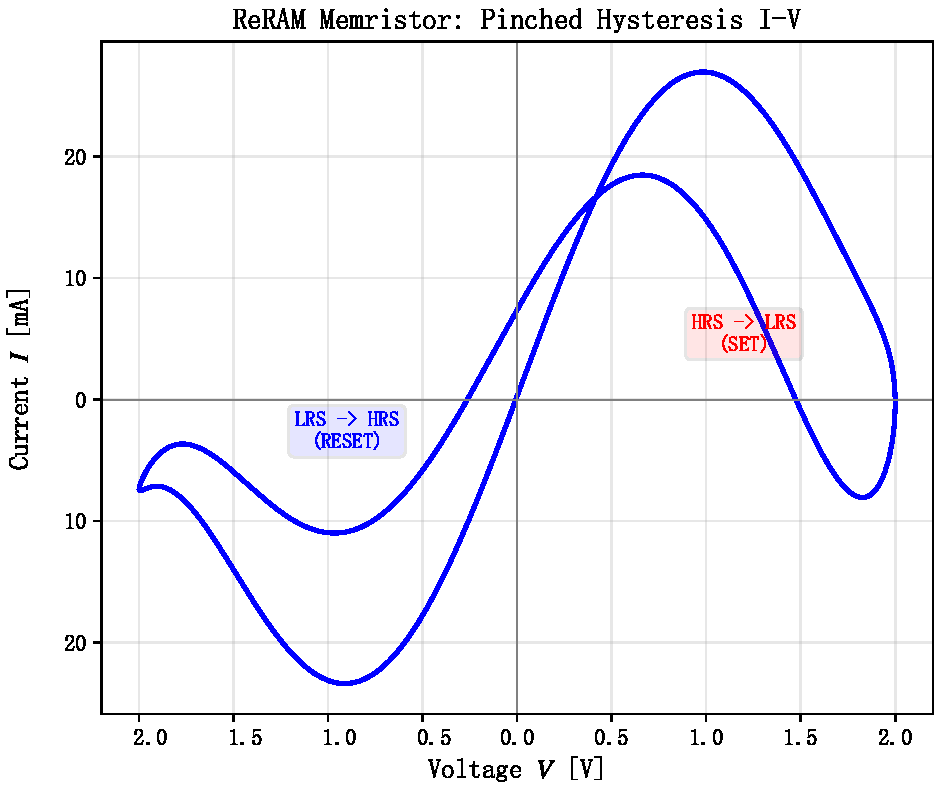
\includegraphics[width=0.55\textwidth]{fig-reram-iv}
\caption{ReRAM忆阻器的I-V捏滞回线。SET（HRS$\to$LRS）
和RESET（LRS$\to$HRS）发生在相反极性的阈值电压处。
回线在原点捏合——忆阻器的定义性特征。}
\label{fig:reram}
\end{figure}

\subsection{逾渗性：随机性的物理根源}

CF的连接/断裂本质上是\textbf{逾渗相变}——在逾渗阈值附近，
CF电导的涨落巨大（临界涨落）。这赋予了ReRAM内禀的随机性：
既是可靠性挑战（阻值读取噪声），也是物理不可克隆函数（PUF）和
真随机数发生器（TRNG）的熵源。

\subsection{ECM/CBRAM}

ECM利用活性金属（Ag, Cu）的电化学溶解/沉积：
阳极：Ag $\to$ Ag$^+$ + e$^-$，
Ag$^+$在电场下穿过固体电解质层$\to$在惰性阴极（Pt, W）上$\to$
Ag$^+$ + e$^-$ $\to$ Ag沉积，形成金属纳米细丝桥接两电极（LRS）。
反向电压使细丝溶解（RESET）。
ECM的开关比$R_{OFF}/R_{ON} > 10^6$，但保持力和耐久性弱于VCM。

\section{相变存储器（PCM）}

\subsection{从光学到电学}

PCM是第4章所述光学相变存储的电气化版本。
存储介质同为GST-225硫系合金，
但写入能量来自焦耳热（$I^2 R$）而非光子吸收，
读取通过电阻对比度（而非反射率对比度）。
晶态（$\sim 10^{-3}$ $\Omega\cdot$cm）与非晶态（$\sim 10^2$ $\Omega\cdot$cm）
的电阻率差异$> 10^5$倍——使PCM可在一个小单元内实现3--4 bits的多级存储。

\begin{figure}[htbp]
\centering
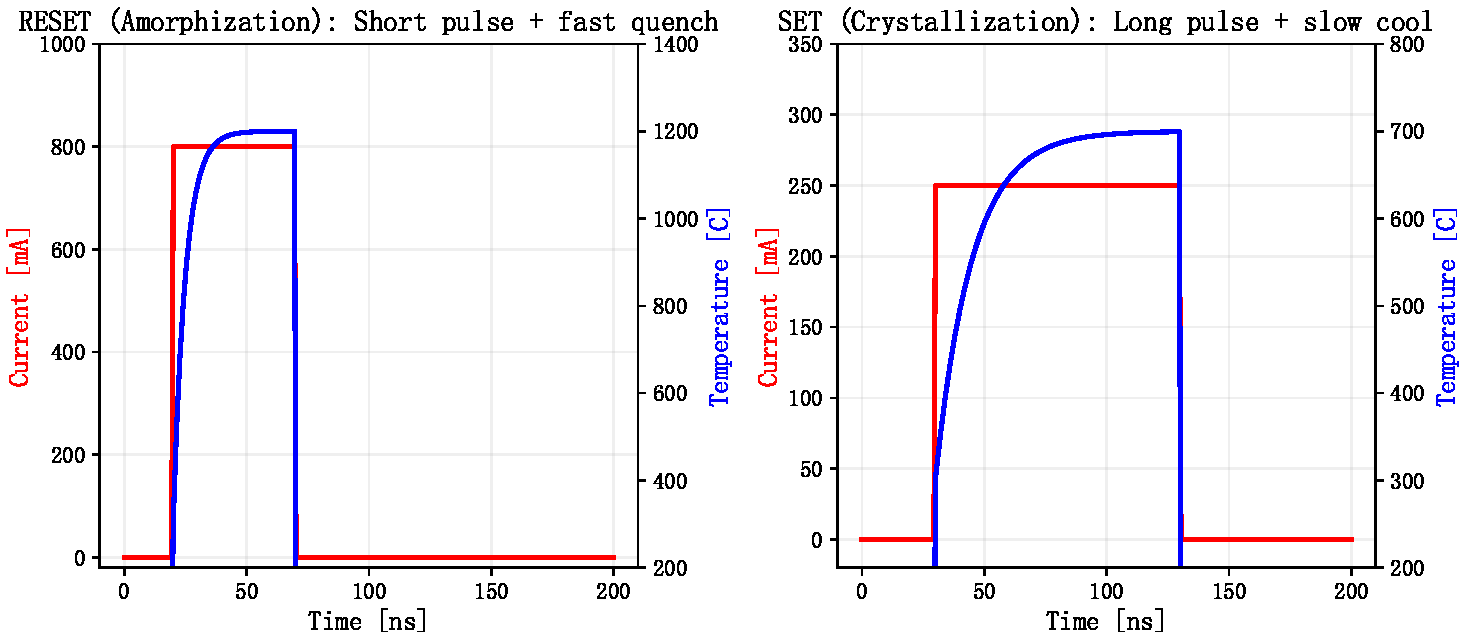
\includegraphics[width=0.9\textwidth]{fig-pcm-pulses}
\caption{PCM的SET/RESET脉冲与温度剖面。
\textbf{左}：RESET——短高电流脉冲（$\sim 800$ $\mu$A, $< 50$ ns）
将GST加热至$> T_m$后急速淬冷，冻结为非晶态（高阻）。
\textbf{右}：SET——较长中等电流脉冲（$\sim 250$ $\mu$A, $\sim 100$ ns）
将GST维持在$T_g$与$T_m$之间的晶化温度窗口，
经JMAK成核-生长晶化为多晶态（低阻）。}
\label{fig:pcm-pulses}
\end{figure}

\subsection{阈值切换与电阻漂移}

PCM的一个关键物理过程是\textbf{阈值切换}——在RESET前，非晶态为高阻，
需要一个临界电压$V_{th}$使电阻骤降，才能馈入大电流达到熔化温度。
两个主导理论：
\begin{enumerate}
  \item \textbf{Poole-Frenkel（PF）发射}：非晶态陷阱的场助热发射导致
  载流子浓度指数增长，当发射增殖至填充陷阱阈值时，载流子雪崩$\to$电阻骤降。
  \item \textbf{临界场模型}：$E_{th} \approx 100$--$200$ MV/m（类击穿）。
\end{enumerate}

PCM的核心可靠性难题是\textbf{电阻漂移}——非晶态GST的结构弛豫
（原子重排以降低能量）导致电阻按幂律增大：
$R(t) \propto t^\nu$，$\nu \approx 0.02$--$0.1$。
对于多级PCM（4 bits/cell），相邻电阻水平的漂移可能在数小时内交叉——
这要求PCM控制器频繁地校准读取参考值。

\section{铁电存储器（FeFET）}

\subsection{铁电极化翻转：KAI动力学}

铁电体是两个自发极化态$\pm P_s$可通过外电场翻转的材料。
翻转动力学由\textbf{Kolmogorov-Avrami-Ishibashi（KAI）模型}描述：
\begin{equation}
  P(t) = P_s\bigl[ 1 - 2\exp(-(t/t_0)^n) \bigr]
\end{equation}
$n \approx 2$--$3$（反向畴成核+生长的有效维度），
$t_0 = t_\infty\exp(E_a/k_B T)$（Arrhenius型）。

2011年发现的HfO$_2$基铁电体（Si:HfO$_2$, Zr:HfO$_2$）是CMOS兼容的
重大突破——在10 nm栅堆叠中保持正交铁电相（$Pca2_1$空间群，$P_s \approx 20$--$30$ $\mu$C/cm$^2$）。

\subsection{FeFET工作原理}

FeFET将MOSFET的栅氧化层替换为铁电层。极化方向通过积累/耗尽效应
调制沟道电导。与NAND闪存相比：写入是压控（非电荷注入，能效更高）、
读取是纯压控电流调制（非破坏性）。
保持力受\textbf{退极化场}限制——铁电层与半导体之间的非零电位移
导致极化随时间半对数衰减（$\propto \log t$）。

\subsection{负电容效应}

在矫顽场附近，铁电自由能-极化曲线上$d^2F/dP^2 < 0$——
对应\textbf{微分负电容}（$C = dQ/dV < 0$）。
将铁电层串联于MOSFET栅堆叠中，可产生电容匹配下的电压放大效应，
有望将亚阈值摆幅降至$< 60$ mV/dec——突破「Boltzmann暴政」。」
这一方案（Salahuddin \& Datta, 2008, Nano Lett.）代表了
「用物理学突破物理极限」的典范。

\section{技术全景对比}

\begin{figure}[htbp]
\centering
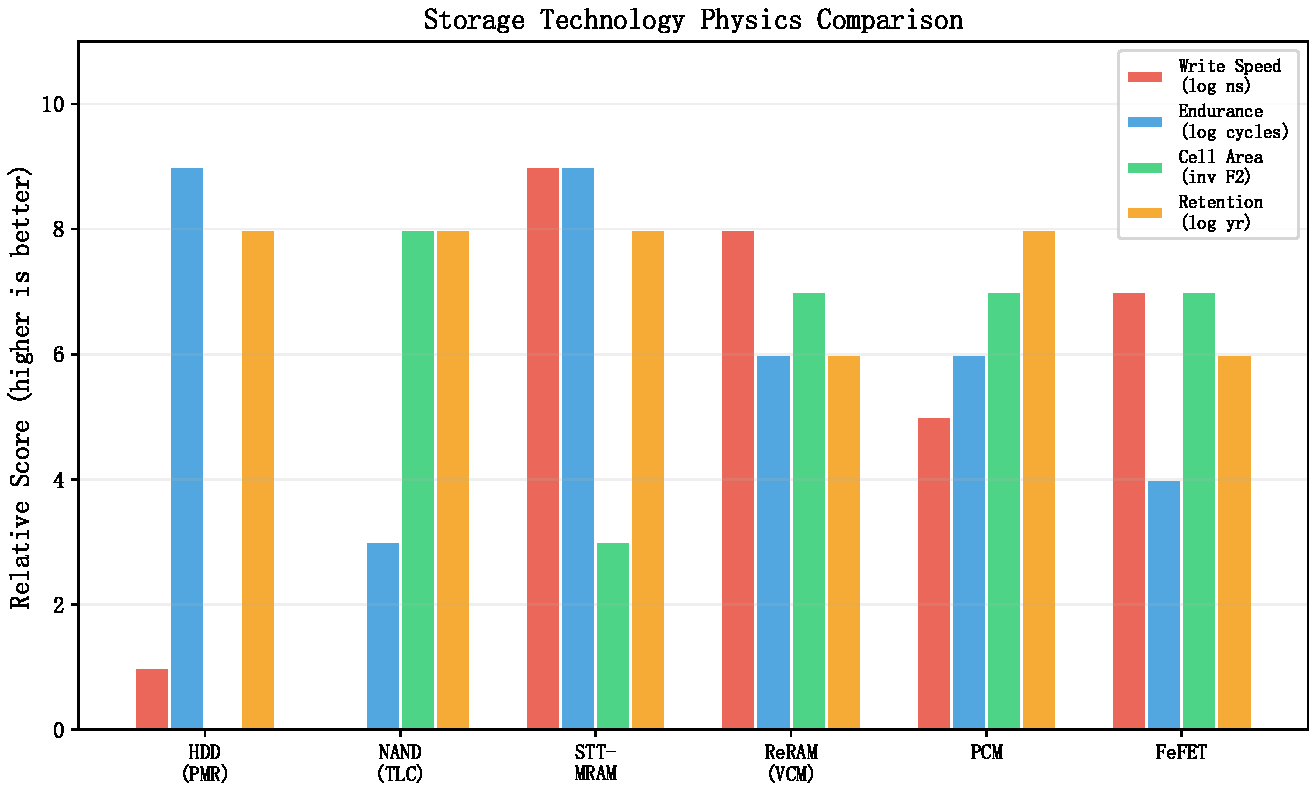
\includegraphics[width=0.9\textwidth]{fig-tech-comparison}
\caption{六种存储技术的四维物理参数对比：
写入速度（对数纳秒）、P/E耐久性（对数循环）、单元面积（倒数$F^2$）、
数据保持力（对数年）。各项越高越好。}
\label{fig:tech-comp}
\end{figure}

\begin{table}[H]
\centering
\caption{新兴存储技术的关键物理参数}
\begin{tabular}{@{}lccccc@{}}
\toprule
技术 & 物理机制 & 单元面积 & 写入时间 & P/E寿命 & 多级能力 \\
\midrule
STT-MRAM & 自旋转移矩 & $\sim 20F^2$ & $\sim 10$ ns & $>10^{12}$ & 2 bits \\
SOT-MRAM & 自旋轨道矩 & $\sim 20F^2$ & $<1$ ns & $>10^{12}$ & 2 bits \\
ReRAM(VCM) & 氧空位迁移 & $\sim 4F^2$ & $\sim 10$ ns & $10^6$--$10^{12}$ & 2--3 bits \\
ReRAM(ECM) & Ag/Cu电化学 & $\sim 4F^2$ & $\sim 10$ ns & $10^4$--$10^6$ & 1 bit \\
PCM & 非晶$\leftrightarrow$晶 & $\sim 4F^2$ & $\sim 50$ ns & $10^7$--$10^8$ & 3--4 bits \\
FeFET & 铁电极化 & $\sim 4F^2$ & $\sim 10$ ns & $10^4$--$10^6$ & 1--2 bits \\
\bottomrule
\end{tabular}
\end{table}

\section{物理机制的统一脉络}

回顾第2章至本章——从磁性存储到铁电存储——可以梳理出一条清晰的物理脉络：

\textbf{存储的本质是将信息编码为某种在室温下具有两个（或多个）稳定可区分状态的
物理量。}这些物理量包括：磁化方向（自旋角动量的集体取向，第2章）、
浮栅电荷数（量子隧穿注入电子数，第3章）、反射率/偏振态（光子-物质相互作用的
宏观光学对比度，第4章）、自旋极化电流（s-d交换的角动量转移）、
氧空位浓度（离子迁移和氧化还原）、晶态/非晶态（相变动力学）、
铁电极化方向（晶胞中离子偏移）。

贯穿所有存储技术的\textbf{物理主线}是：
\begin{enumerate}
  \item \textbf{能垒} $E_B \gg k_B T$ 确保非易失性——
  Arrhenius定律$\tau = \tau_0\exp(E_B/k_B T)$。
  \item \textbf{写入操作}必须以合理的能量和时间跨越这个能垒。
  \item \textbf{读取操作}必须无损地（或低损地）区分这些状态。
\end{enumerate}

这个「三元要求」——稳定性、可写性、可读性——是所有存储技术的物理公分母。

% ===================================================================
% CHAPTER 6
% ===================================================================
\chapter{删除、残留与擦除}
\label{ch:deletion}

\section{五个物理问题的汇聚}

前五章建立了数据存储的完整物理框架。
本章将全部物理知识汇聚至一个对信息安全具有根本重要性的问题：

\begin{quote}
\textbf{当我们在计算机上点击「删除」时，存储介质中到底发生了什么物理变化？}
\end{quote}

答案——令人不安地——是：\textbf{几乎什么物理变化都没有}。
文件删除只修改了文件系统的元数据（目录项、inode、分配位图）；
快速格式化仅重建了空文件系统的超级块；
SSD上的TRIM/UNMAP指令仅向FTL发送了「此LBA范围不再需要」的逻辑通知。

在物理层面——磁畴方向未变（HDD）、浮栅电荷未变（NAND闪存）、
反射率对比未变（光盘）、极化方向未变（FeFET）——
信息完好无损地存在于介质中，只是失去了文件系统的索引。

本章从每一种存储技术的微观物理出发，
定量分析「删除」操作的真实物理后果、
物理残留给数据恢复提供的可能途径、
以及真正安全擦除的物理极限——从Landauer原理给出的热力学下界到
AES-256加密擦除的计算安全保证。

\section{HDD：删除、覆写与剩磁}

\subsection{文件系统层的「删除」}

文件系统删除仅改变了三个数据结构：
文件名首字节被改写为特殊标记（如FAT中的0xE5）、
空间分配位图中该文件占用的簇被标记为「空闲」、
inode状态字段更新。盘片上对应扇区的磁化方向——百亿个CoCrPt晶粒的
$\mathbf{m} = \pm\hat{z}$模式——\textbf{纹丝未动}。

快速格式化只是更大范围的同质操作：文件系统元数据结构（超级块、位图、
目录树）被重建为初始状态。所有先前的数据扇区原封不动——
如同将一本书的目录页撕掉并打印上新的目录，
而正文的每一页完好无损地留在原处。

\subsection{覆写后的剩磁}

单次覆写（将新数据写入之前有旧数据的扇区）确实翻转了大部分晶粒的磁化方向——
但并非100\%完美。两种不完备机制：

\textbf{(1) 写头位置偏离（Misregistration）}。
写磁头每次定位存在随机偏差。对于道间距50--70 nm的现代HDD，
$\pm 3$ nm（$3\sigma$）的偏离在磁道边缘留下前次写入磁化的残留。

\textbf{(2) 不完全磁化翻转}。
在写场梯度区（$H_z < H_K$的磁道边缘区域），处于高矫顽力尾部的晶粒
（由晶粒尺寸和各向异性分布引起）可能未被完全翻转。
微磁学模拟表明：对$H_{\text{write}}/H_K \approx 1.5$的典型写场，
未翻转晶粒比例约为$10^{-4}$--$10^{-3}$。

覆写后剩磁信号相对于原始写信号的衰减：
\begin{equation}
  \text{SNR}_{\text{remanent}} \approx -20\log_{10}\!\left(
    \frac{2\sigma_{\text{misreg}}}{W} + f_{\text{unswitched}} \right)
  \approx -30\ \text{to}\ -40\ \text{dB}
\end{equation}

\textbf{对现代PMR HDD的评估}：单次覆写后的剩磁信噪比（$\lesssim -30$ dB）
已低于实用恢复的门槛（$\sim -25$ dB，受限于MFM噪声底）。
NIST SP 800-88 Rev.1（2014）因此建议对现代HDD仅执行单次覆写。
但从严格的物理学角度——\textbf{绝对的安全不存在，只存在
「在给定攻击预算下不可行」的安全}。

\subsection{剩磁的探测：MFM原理与限制}

磁力显微镜（MFM）是检测剩磁的核心工具。两级扫描原理：
形貌扫描（探针近距离轻敲模式）获得表面地形，
磁力扫描（探针抬升至50--100 nm高度）通过共振频率偏移
$\Delta f = -(f_0/2k)\,\partial F_z/\partial z$检测磁力梯度。

\textbf{现实约束}：对现代4 TB HDD（$\sim 3 \times 10^{13}$个晶粒簇），
全盘MFM扫描在可行时间尺度内（$<1$年）不可行。
MFM剩磁恢复主要用于微区取证（$\mu$m$^2$级），而非全盘数据重建。

\section{NAND闪存：FTL异地更新与GC延迟}

\subsection{逻辑删除的物理真相}

TRIM/UNMAP命令的实际物理后果：FTL收到「LBA $X$不再需要「后，
仅将对应物理页在映射表中标记为」无效（stale）」。」
该页的浮栅电荷\textbf{完好无损}——电子安稳地存储在被绝缘体包围的浮栅中，
其热力学保持时间从最初编程时刻起算（而非从逻辑删除时刻起算）。

GC（垃圾回收）的延迟造成了不可预测的数据残留窗口：
\begin{itemize}
  \item SSD空闲空间充足（$>30\%$）时，GC可能懒惰运行——无效页保留数周至数月。
  \item TRIM仅通知FTL——GC何时真正擦除该块完全由固件决定，不可预测。
  \item 企业级SSD的GC可能激进（后台持续回收），消费级SSD的GC在空闲时触发。
\end{itemize}

\subsection{物理恢复路径}

通过绕过FTL直接读取NAND物理页可恢复TRIM后的数据：
\begin{itemize}
  \item \textbf{芯片拆卸+NAND编程器}：将NAND芯片从SSD PCB焊下，
  通过专用编程器逐块/逐页读取原始数据（16 KB页数据+元数据+ECC）。
  \item \textbf{JTAG/调试接口}：对SSD控制器进行固件级调试，暴露FTL映射表。
\end{itemize}

技术挑战：控制器的LFSR加扰（降低CCI、平衡磨损）和硬件加密（SED, AES-256-XTS）。

\subsection{安全擦除：两种物理路径}

\textbf{(1) 物理块擦除}（ATA Secure Erase）：对所有用户块执行FN隧穿擦除，
$V_{th}$分布全部恢复至擦除态。耗时$\sim 1$--$5$ min/TB。

\textbf{(2) 加密擦除}（Cryptographic Erase）：仅销毁内部介质加密密钥（MEK）。
所有数据即刻变为不可解密的AES-256密文。耗时$< 1$秒。

\textbf{加密擦除是当前最可靠且最高效的数据清除方案。}
AES-256密钥空间为$2^{256} \approx 1.16 \times 10^{77}$——
暴力破解所需计算时间远超宇宙年龄（$\sim 10^{10}$年）。

\begin{physbox}
\textbf{物理块擦除后的极限理论残余。}
经历数千次P/E循环后，氧化层深陷阱（能级$> 1.5$ eV）中的「固定」电荷
可能不被常规擦除操作完全清除。这些电荷与原始数据的关系目前无任何已知提取方法。
从信息论角度——物理系统中不存在绝对事件——概率并非严格为零，
但距离任何可设想的恢复技术远超过当前和可预见未来的技术能力。
\end{physbox}

\section{Landauer原理：信息擦除的热力学下界}

\subsection{物理极限}

Rolf Landauer（1961）从热力学和信息论推导了信息擦除的终极物理极限：
\begin{equation}\label{eq:landauer}
  \boxed{ \Delta E_{\text{min}} = k_B T \ln 2 }
\end{equation}
在室温下（$T = 300$ K）：
$\Delta E_{\text{min}} \approx 2.87 \times 10^{-21}$ J $\approx 18$ meV。

\textbf{这个值极小}——现代器件每比特实际擦除能耗高出$10^5$--$10^8$倍。
但其\textbf{理论意义}深远：

\begin{itemize}
  \item 信息擦除（$2^N \to 1$的映射）本质不可逆——它必然将相空间体积减半，
  从而增加环境熵$\Delta S \ge k_B\ln 2$（每比特），对应最小热耗散
  $T\Delta S = k_B T\ln 2$。
  \item Landauer极限是\textbf{任何物理擦除机制的热力学下界}——
  无论磁化翻转、电荷隧穿、铁电极化切换还是相变转换。
  \item 该极限已在实验中被验证（B\'{e}rut et al., 2012, Nature）。
\end{itemize}

\begin{figure}[htbp]
\centering
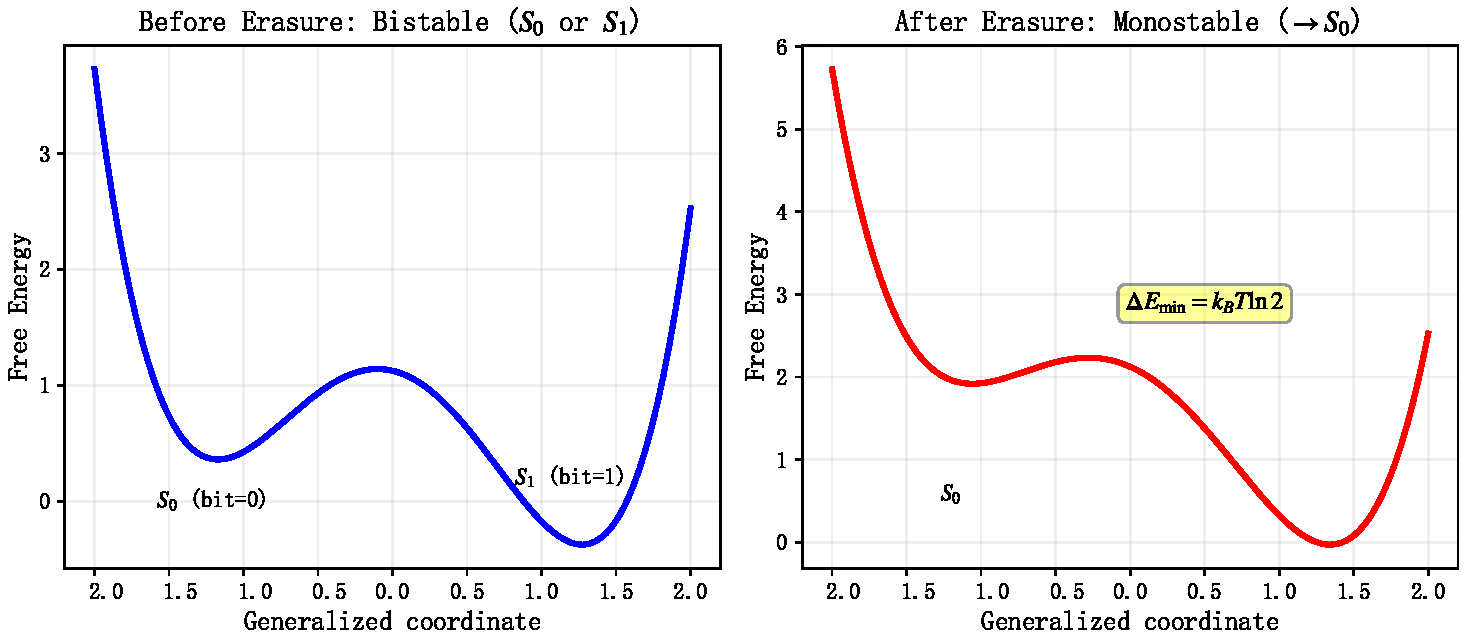
\includegraphics[width=0.9\textwidth]{fig-landauer}
\caption{Landauer原理的能景示意图。
\textbf{左}：擦除前——双阱势，系统可处于$S_0$（bit=0）或$S_1$（bit=1）。
任意一个宏观状态对应两个微观可能——信息容量为1 bit。
\textbf{右}：擦除后——单阱势，系统强制收敛至$S_0$。
相空间体积减半，环境熵增加$\Delta S = k_B\ln 2$，
对应最小热耗散$T\Delta S = k_B T\ln 2 \approx 18$ meV/bit。}
\label{fig:landauer-fig}
\end{figure}

\subsection{信息残留的统计量化：KL散度}

从统计物理角度，「完全擦除」是概率概念而非二值状态。
设擦除前比特为$X \in \{0,1\}$，擦除后物理状态$S$的分布为$\rho_{\text{final}}(S)$。
信息残留可用$X$与$S$之间的\textbf{互信息}（Kullback-Leibler散度的一个规范形式）严格量化：
\begin{equation}\label{eq:kl}
  I(X;S) = D_{KL}\!\left( P(X,S)\,\|\,P(X)P(S) \right)
\end{equation}
$I(X;S) \to 0$：擦除后的状态与原始比特统计独立，擦除「物理完全」。
Chernoff-Stein引理：以错误概率$\alpha$检测残留所需的独立测量次数$N$满足
$N \sim |\ln\alpha| / I(X;S)$——$I(X;S)$越小，「恢复」所需的统计样本越多。

\textbf{可达到的极限}：在有限能量和有限时间内，$I(X;S)$永远不能严格为零，
但可以降至「对任何可设想的攻击预算无法检测」的程度。
这是现代安全擦除标准的物理理论基础。

\section{安全擦除的物理可靠级}

\begin{table}[H]
\centering
\caption{各介质安全擦除的物理评估}
\begin{tabular}{@{}p{2.5cm}p{4.5cm}p{5cm}p{2.5cm}@{}}
\toprule
介质 & 最可靠方法 & 物理基础 & 可靠级 \\
\midrule
HDD & 单次全覆写+验证 & 改变所有扇区磁畴；剩磁SNR $< -30$ dB & 实用安全 \\
HDD & 物理粉碎（颗粒$< 2$ mm） & 晶粒间物理对应关系不可逆混淆 & 绝对安全 \\
SSD（无加密）& Secure Erase & FN隧穿擦除所有浮栅电荷 & 高度可靠$^\dagger$ \\
SSD（加密） & 加密擦除（销毁MEK） & AES-256密钥销毁$\to$不可解密密文 & 最可靠+最快 \\
光盘（ROM） & 物理破坏 & 反射坑结构不可逆损坏 & 绝对安全 \\
光盘（RW） & 全盘覆写+验证 & 全部非晶标记重写 & 实用安全 \\
PCM/ReRAM & 全阵列SET/RESET & 所有单元切换至统一态 & 需验证$^\ddagger$ \\
\bottomrule
\end{tabular}

\vspace{4pt}
{\footnotesize
$^\dagger$ 无已知物理恢复方法。但深能级陷阱固定电荷在理论上不能绝对排除。
$^\ddagger$ 新兴存储的擦除完全性研究远不如HDD/SSD充分，建议配套加密措施。}
\end{table}

\section{结语：物理的边界}

我们从苏美尔泥板的塑性形变出发，穿越了海森堡交换作用、Stoner-Wohlfarth翻转、
Fowler-Nordheim量子隧穿、MgO Bloch态对称性筛选、
GST相变动力的JMAK方程和ReRAM氧空位细丝的逾渗相变，
最终抵达Landauer在1961年揭示的不可规避的事实：

\textbf{擦除1比特信息在物理上不可能以低于$k_B T\ln 2$的能量完成，
且在有限能量/时间内，擦除永远无法「绝对完全」。」}

这个结论不是工程限制——它是热力学和信息论交汇处的基本物理定律。
它直接意味着：\textbf{任何「安全删除」的声明，
本质上都是」在给定的攻击预算下不可恢复」的陈述，
而非「信息已从宇宙中消失」的形而上学断言}。

存储物理的深层美感在于：
同一个Arrhenius定律$\tau = \tau_0\exp(E_B/k_B T)$同时支配着
硬盘的数据保持（$E_B = K_u V$）、闪存的电荷保持（$E_B \approx 1.0$--$1.2$ eV）、
以及所有新兴存储中磁化/空位/极化态的热稳定性。
同一个量子隧穿机制（FN的WKB积分）同时负责闪存的写入、擦除和
（在氧化层退化后的）电荷泄漏。
同一个信息论约束（Landauer原理）为所有物理擦除机制设定了不可逾越的热力学下界。

\textbf{物理学是存储技术上不可绕过的第一语言。}
理解它，我们就理解了数据从何而来，归于何处——以及中间每一步的物理代价。

\vspace{1cm}
\begin{flushright}
——全书完——
\end{flushright}

% ===================================================================
\appendix
\chapter{物理常数与材料参数}

\begin{table}[H]
\centering
\caption{通用物理常数}
\begin{tabular}{@{}lll@{}}
\toprule
常数 & 符号 & 值 \\
\midrule
Bohr磁子 & $\mu_B$ & $9.274 \times 10^{-24}$ J/T \\
Boltzmann常数 & $k_B$ & $1.381 \times 10^{-23}$ J/K \\
基本电荷 & $e$ & $1.602 \times 10^{-19}$ C \\
Planck常数 & $h$ & $6.626 \times 10^{-34}$ J$\cdot$s \\
约化Planck常数 & $\hbar$ & $1.055 \times 10^{-34}$ J$\cdot$s \\
自由电子旋磁比 & $\gamma_e$ & $1.761 \times 10^{11}$ rad/(s$\cdot$T) \\
真空磁导率 & $\mu_0$ & $4\pi \times 10^{-7}$ N/A$^2$ \\
真空介电常数 & $\varepsilon_0$ & $8.854 \times 10^{-12}$ F/m \\
自由电子质量 & $m_e$ & $9.109 \times 10^{-31}$ kg \\
电子伏特 & eV & $1.602 \times 10^{-19}$ J \\
量子电导 & $G_0 = 2e^2/h$ & $(12.906\text{ k}\Omega)^{-1}$ \\
Landauer能量 & $k_B T\ln 2$ @300K & $2.87 \times 10^{-21}$ J $= 18$ meV \\
\bottomrule
\end{tabular}
\end{table}

\begin{table}[H]
\centering
\caption{各技术的核心材料参数}
\begin{tabular}{@{}llll@{}}
\toprule
参数 & 符号 & 典型值 & 出处 \\
\midrule
CoCrPt各向异性能密度 & $K_u$ & $(2\text{--}5)\times 10^5$ J/m$^3$ & 第2章 \\
FePt($L1_0$)各向异性能密度 & $K_u$ & $7\times 10^6$ J/m$^3$ & 第2章(HAMR) \\
Co交换刚度 & $A$ & $3.0\times 10^{-11}$ J/m & 第2章 \\
Co饱和磁化 & $M_s$ & $1.42 \times 10^6$ A/m & 第2章 \\
Gilbert阻尼(CoCrPt) & $\alpha$ & 0.02--0.05 & 第2,5章 \\
MgO隧穿势垒高度 & $\phi_B$ & 3.15 eV & 第2章 \\
SiO$_2$电子有效质量 & $m_{ox}^*$ & $0.42\,m_e$ & 第3章 \\
隧穿氧化层厚度 & $t_{tun}$ & 5--7 nm & 第3章 \\
控制栅耦合比 & $\alpha_{CG}$ & 0.50--0.65 & 第3章 \\
数据保持激活能 & $E_a$ & 1.0--1.2 eV & 第3章 \\
GST-225熔点 & $T_m$ & $\sim 610^\circ$C & 第4,5章 \\
GST玻璃转变温度 & $T_g$ & $\sim 150^\circ$C & 第4,5章 \\
自旋Hall角($\beta$-W) & $\theta_{SH}$ & 0.3--0.5 & 第5章 \\
\bottomrule
\end{tabular}
\end{table}

% ===================================================================
\begin{thebibliography}{99}

\bibitem{shannon48}
C.~E.~Shannon, ``A mathematical theory of communication,''
\textit{Bell Syst.\ Tech.\ J.}, vol.\ 27, pp.\ 379--423, 623--656, 1948.
\href{https://doi.org/10.1002/j.1538-7305.1948.tb01338.x}{doi:10.1002/j.1538-7305.1948.tb01338.x}

\bibitem{aharoni}
A.~Aharoni, \textit{Introduction to the Theory of Ferromagnetism}, 2nd ed.\
Oxford University Press, 2000.
\href{https://scholar.google.com/scholar?q=Introduction+to+the+Theory+of+Ferromagnetism+Aharoni}{Google Scholar}

\bibitem{brown}
W.~F.~Brown, Jr., \textit{Micromagnetics}.\ Interscience, 1963.
\href{https://scholar.google.com/scholar?q=Micromagnetics+Brown+1963}{Google Scholar}

\bibitem{stoner48}
E.~C.~Stoner and E.~P.~Wohlfarth, ``A mechanism of magnetic hysteresis
in heterogeneous alloys,''
\textit{Phil.\ Trans.\ R.\ Soc.\ Lond.\ A}, vol.\ 240, pp.\ 599--642, 1948.
\href{https://doi.org/10.1098/rsta.1948.0007}{doi:10.1098/rsta.1948.0007}

\bibitem{neel49}
L.~N\'{e}el, ``Th\'{e}orie du tra\^{i}nage magn\'{e}tique des
ferromagn\'{e}tiques en grains fins,''
\textit{Ann.\ G\'{e}ophys.}, vol.\ 5, pp.\ 99--136, 1949.
\href{https://scholar.google.com/scholar?q=Neel+trainage+magnetique+ferromagnetiques+grains+fins+1949}{Google Scholar}

\bibitem{bertram}
H.~N.~Bertram, \textit{Theory of Magnetic Recording}.\
Cambridge University Press, 1994.
\href{https://doi.org/10.1017/CBO9780511623066}{doi:10.1017/CBO9780511623066}

\bibitem{slonczewski96}
J.~C.~Slonczewski, ``Current-driven excitation of magnetic multilayers,''
\textit{J.\ Magn.\ Magn.\ Mater.}, vol.\ 159, pp.\ L1--L7, 1996.
\href{https://doi.org/10.1016/0304-8853(96)00062-5}{doi:10.1016/0304-8853(96)00062-5}

\bibitem{butler01}
W.~H.~Butler et al., ``Spin-dependent tunneling conductance of
Fe$|$MgO$|$Fe sandwiches,''
\textit{Phys.\ Rev.\ B}, vol.\ 63, 054416, 2001.
\href{https://doi.org/10.1103/PhysRevB.63.054416}{doi:10.1103/PhysRevB.63.054416}

\bibitem{parkin04}
S.~S.~P.~Parkin et al., ``Giant tunnelling magnetoresistance at room
temperature with MgO (100) tunnel barriers,''
\textit{Nature Materials}, vol.\ 3, pp.\ 862--867, 2004.
\href{https://doi.org/10.1038/nmat1256}{doi:10.1038/nmat1256}

\bibitem{kryder08}
M.~H.~Kryder et al., ``Heat assisted magnetic recording,''
\textit{Proc.\ IEEE}, vol.\ 96, pp.\ 1810--1835, 2008.
\href{https://doi.org/10.1109/JPROC.2008.2004315}{doi:10.1109/JPROC.2008.2004315}

\bibitem{bez03}
R.~Bez, E.~Camerlenghi, and A.~Modelli, ``Introduction to flash memory,''
\textit{Proc.\ IEEE}, vol.\ 91, pp.\ 489--502, 2003.
\href{https://doi.org/10.1109/JPROC.2003.811702}{doi:10.1109/JPROC.2003.811702}

\bibitem{lenzlinger69}
M.~Lenzlinger and E.~H.~Snow, ``Fowler-Nordheim tunneling into
thermally grown SiO$_2$,''
\textit{J.\ Appl.\ Phys.}, vol.\ 40, pp.\ 278--283, 1969.
\href{https://doi.org/10.1063/1.1657811}{doi:10.1063/1.1657811}

\bibitem{prall07}
K.~Prall, ``Scaling non-volatile memory below 30nm,''
\textit{IEEE NVMTS}, pp.\ 5--10, 2007.
\href{https://scholar.google.com/scholar?q=Prall+scaling+non-volatile+memory+below+30nm}{Google Scholar}

\bibitem{cai12}
Y.~Cai et al., ``Error patterns in MLC NAND flash memory,''
\textit{Proc.\ DATE}, pp.\ 521--526, 2012.
\href{https://doi.org/10.1109/DATE.2012.6176524}{doi:10.1109/DATE.2012.6176524}

\bibitem{micheloni10}
R.~Micheloni and L.~Crippa, \textit{Inside NAND Flash Memories}.\
Springer, 2010.
\href{https://doi.org/10.1007/978-90-481-9431-5}{doi:10.1007/978-90-481-9431-5}

\bibitem{born99}
M.~Born and E.~Wolf, \textit{Principles of Optics}, 7th ed.\
Cambridge University Press, 1999.
\href{https://doi.org/10.1017/CBO9781139644181}{doi:10.1017/CBO9781139644181}

\bibitem{richards59}
B.~Richards and E.~Wolf, ``Electromagnetic diffraction in optical
systems II,''
\textit{Proc.\ Roy.\ Soc.\ A}, vol.\ 253, pp.\ 358--379, 1959.
\href{https://doi.org/10.1098/rspa.1959.0200}{doi:10.1098/rspa.1959.0200}

\bibitem{yamada91}
N.~Yamada et al., ``Rapid-phase transitions of GeTe-Sb$_2$Te$_3$
pseudobinary amorphous thin films,''
\textit{J.\ Appl.\ Phys.}, vol.\ 69, pp.\ 2849--2856, 1991.
\href{https://doi.org/10.1063/1.348620}{doi:10.1063/1.348620}

\bibitem{kogelnik69}
H.~Kogelnik, ``Coupled wave theory for thick hologram gratings,''
\textit{Bell Syst.\ Tech.\ J.}, vol.\ 48, pp.\ 2909--2947, 1969.
\href{https://doi.org/10.1002/j.1538-7305.1969.tb01198.x}{doi:10.1002/j.1538-7305.1969.tb01198.x}

\bibitem{chua71}
L.~O.~Chua, ``Memristor---The missing circuit element,''
\textit{IEEE Trans.\ Circuit Theory}, vol.\ 18, pp.\ 507--519, 1971.
\href{https://doi.org/10.1109/TCT.1971.1083337}{doi:10.1109/TCT.1971.1083337}

\bibitem{strukov08}
D.~B.~Strukov et al., ``The missing memristor found,''
\textit{Nature}, vol.\ 453, pp.\ 80--83, 2008.
\href{https://doi.org/10.1038/nature06932}{doi:10.1038/nature06932}

\bibitem{waser09}
R.~Waser et al., ``Redox-based resistive switching memories,''
\textit{Adv.\ Mater.}, vol.\ 21, pp.\ 2632--2663, 2009.
\href{https://doi.org/10.1002/adma.200900375}{doi:10.1002/adma.200900375}

\bibitem{burr10}
G.~W.~Burr et al., ``Phase change memory technology,''
\textit{J.\ Vac.\ Sci.\ Technol.\ B}, vol.\ 28, pp.\ 223--262, 2010.
\href{https://doi.org/10.1116/1.3301579}{doi:10.1116/1.3301579}

\bibitem{boscke11}
T.~S.~B\"{o}scke et al., ``Ferroelectricity in hafnium oxide thin films,''
\textit{Appl.\ Phys.\ Lett.}, vol.\ 99, 102903, 2011.
\href{https://doi.org/10.1063/1.3634052}{doi:10.1063/1.3634052}

\bibitem{salahuddin08}
S.~Salahuddin and S.~Datta, ``Use of negative capacitance to provide
voltage amplification for low power nanoscale devices,''
\textit{Nano Lett.}, vol.\ 8, pp.\ 405--410, 2008.
\href{https://doi.org/10.1021/nl071804g}{doi:10.1021/nl071804g}

\bibitem{landauer61}
R.~Landauer, ``Irreversibility and heat generation in the computing
process,''
\textit{IBM J.\ Res.\ Dev.}, vol.\ 5, pp.\ 183--191, 1961.
\href{https://doi.org/10.1147/rd.51.0183}{doi:10.1147/rd.51.0183}

\bibitem{berut12}
A.~B\'{e}rut et al., ``Experimental verification of Landauer's principle
linking information and thermodynamics,''
\textit{Nature}, vol.\ 483, pp.\ 187--189, 2012.
\href{https://doi.org/10.1038/nature10872}{doi:10.1038/nature10872}

\bibitem{cover91}
T.~M.~Cover and J.~A.~Thomas, \textit{Elements of Information Theory}.\
Wiley, 1991.
\href{https://doi.org/10.1002/047174882X}{doi:10.1002/047174882X}

\bibitem{gutmann96}
P.~Gutmann, ``Secure deletion of data from magnetic and solid-state
memory,''
\textit{Proc.\ 6th USENIX Security Symp.}, pp.\ 77--89, 1996.
\href{https://www.usenix.org/legacy/publications/library/proceedings/sec96/full_papers/gutmann/}{usenix.org}

\bibitem{wright08}
C.~Wright, D.~Kleiman, and S.~Sundhar, ``Overwriting hard drive data:
The great wiping controversy,''
\textit{LNCS}, vol.\ 5352, pp.\ 243--257, 2008.
\href{https://doi.org/10.1007/978-3-540-89862-7_21}{doi:10.1007/978-3-540-89862-7\_21}

\bibitem{wei11}
M.~Wei et al., ``Reliably erasing data from flash-based solid state
drives,''
\textit{Proc.\ 9th USENIX FAST}, pp.\ 105--117, 2011.
\href{https://www.usenix.org/conference/fast11/reliably-erasing-data-flash-based-solid-state-drives}{usenix.org}

\bibitem{nist14}
R.~Kissel et al., ``Guidelines for Media Sanitization,''
\textit{NIST SP 800-88}, Rev.\ 1, 2014.
\href{https://doi.org/10.6028/NIST.SP.800-88r1}{doi:10.6028/NIST.SP.800-88r1}


\bibitem{kukhtarev79}
N.~V.~Kukhtarev et al., ``Holographic storage in electrooptic
crystals,''
\textit{Ferroelectrics}, vol.\ 22, pp.\ 949--960, 1979.
\href{https://doi.org/10.1080/00150107908239450}{doi:10.1080/00150107908239450}

\end{thebibliography}

\end{document}
